\documentclass[12pt]{iopart}
\pdfminorversion=4
%Uncomment next line if AMS fonts required
%\usepackage{iopams}
\usepackage{myphysics} %units, particles and misc definitions from ATLAS
\usepackage{graphicx}  %\includegraphics...

\begin{document}

\title[Electroweak phyiscs at the LHC]{Electroweak physics at the LHC}
\author{J Berryhill$^1$ and A Oh$^2$}

\address{$^1$ Fermi National Accelerator Laboratory, Batavia, IL, USA}
\address{$^2$ School of Physics and Astronomy, University of Manchester, Manchester, UK}

%\ead{submissions@iop.org}
%\vspace{10pt}
%\begin{indented}
%\item[]February 2014
%\end{indented}

\begin{abstract}
The Large Hadron Collider (LHC) has completed in 2012 its first
running phase and the experiments have collected data sets of pp
collisions at center-of-mass energies of 7 and 8 \TeV\xspace with an
integrated luminosity of about 5 \ifb and 20 \ifb, respectively.  Analyses
of these data sets have produced a rich set of results in the
electroweak sector of the standard model. This article reviews the
status of electroweak measurements of the ATLAS and CMS experiments at
the LHC and discusses phenomenological developments in the electroweak
sector.
\end{abstract}

% Uncomment for PACS numbers
\pacs{12.15.-y, 12.60.Cn, 14.70.-e}
%
% Uncomment for keywords
%\vspace{2pc}
%\noindent{\it Keywords}: XXX, YYY, ZZZ
%
% Uncomment for Submitted to journal title message
\submitto{\jpg}
%
% Uncomment if a separate title page is required
\maketitle
%
% For two-column output uncomment the next line and choose [10pt] rather than [12pt] in the \documentclass declaration
%\ioptwocol
%


\section{Introduction}
\subsection{Motivation to study the electroweak sector}
\subsection{Electroweak physics at hadron colliders}
\subsection{LHC physics program}
\subsection{Electroweak challenges for Run 2 and beyond}

\section{Theory overview and recent developments}
\subsection{PDF and electroweak observables (V+jets, $\phi^*$)}
\subsection{Electroweak NLO corrections}
\subsection{Anomalous gauge couplings and effective field theory}
\subsection{Oblique corrections, constructed observables}


\section{Inclusive boson production}
\subsection{Drell-Yan production}
\label{ss-inclboson-drellyan}
At a hadron collider, the most fundamental tests of electroweak boson
couplings to fermions are measurements of the kinematic properties of
Drell-Yan (DY) lepton pair production.  At leading order, Drell-Yan
production occurs when a quark--anti-quark pair in the initial state
annihilates into an electroweak boson, which subsequently decays to a
lepton pair. Differential cross section calculations exist for
next-to-next-to leading order (NNLO) QCD corrections as well as NLO
electroweak corrections. In the EFT context, such a process is
sensitive to four-fermion contact interactions of the type

\begin{equation}\label{lagrangian}
\begin{array}{r@{\,}c@{}c@{\,}l@{\,}l}
\mathcal L = \frac{g^2}{\Lambda^2}\;[ && \eta_{\rm LL}&\, (\overline q_{\rm L}\gamma_{\mu} q_{\rm L})\,(\overline\ell_{\rm L}\gamma^{\mu}\ell_{\rm L}) \nonumber \\
& +&\eta_{\rm RR}& (\overline q_{\rm R}\gamma_{\mu} q_{\rm R}) \,(\overline\ell_{\rm R}\gamma^{\mu}\ell_{\rm R}) \\
&+&\eta_{\rm LR}& (\overline q_{\rm L}\gamma_{\mu} q_{\rm L}) \,(\overline\ell_{\rm R}\gamma^{\mu}\ell_{\rm R}) \\
&+&\eta_{\rm RL}& (\overline q_{\rm R}\gamma_{\mu} q_{\rm R}) \,(\overline\ell_{\rm L}\gamma^{\mu}\ell_{\rm L})& ] \: ,\nonumber
\end{array}
\end{equation}
where $g$ is a coupling constant, $\Lambda$ is the contact interaction scale,
and $q_{\rm L,R}$ and $\ell_{\rm L,R}$ are left-handed and right-handed quark and
lepton fields, respectively. The parameters $\eta_{i,j}$ denote the relative interference of the operators;
the experiments have considered the cases $\eta_{\rm LR} = \eta_{\rm RL} = \pm 1$,
$\eta_{\rm LL} = \pm 1$, or $\eta_{\rm RR} = \pm 1$.

Experiments select electron or muon pairs above trigger thresholds:
CMS selects leading lepton $\pt >$ 17 GeV and second leading lepton
$\pt >$ 8 GeV inclusively, and ATLAS selects high mass events with
both lepton $\pt >$ 25 GeV.  Backgrounds to Drell-Yan production are
relatively small, and consist of real prompt lepton pair production
from top quark or boson pairs, as well as fake electrons from QCD
jets.  The real lepton pair background is flavor democratic, and can
therefore be reliably estimated from $e\mu$ pair production.  Fake
electron production is typically estimated from background enriched
QCD jet samples, from which the fake electron rate can be measured,
convolved with electron-jet control samples.

Figure~\ref{fig:ss-inclboson-drellyan-atlas7tev} shows the Drell-Yan
cross section at high electron pair mass measured by ATLAS at 7
TeV~\cite{Aad:2013iua}.  The cross section uncertainty is
predominantly systematic below 400 GeV in pair mass and predominantly
statistical above 400 GeV.  The data are compared with an NNLO QCD
prediction with NLO electroweak corrections, provided by the
\texttt{FEWZ} 3.1
generator~\cite{Melnikov:2006kv,Gavin:2010az,Li:2012wna}.  The
prediction also includes photon induced lepton pair production, which
generally increases cross section estimates by a few percent. The
\texttt{FEWZ} prediction generally underestimates the cross section,
however a correlated chi-squared analysis concludes that this is not
statistically significant.

Figure~\ref{fig:ss-inclboson-drellyan-cms8tev} shows the Drell-Yan
cross section for electron or muon pairs measured by CMS at 8
TeV~\cite{CMS:2014jea}.  Agreement with the \texttt{FEWZ} prediction
is observed over the entire measured mass range, from 15 GeV to 2000
GeV.  CMS has also measured the double differential cross section with
respect to dilepton rapidity in several bins of dilepton mass, as well
as a differential cross section ratio between the 8 TeV and 7 TeV
data, which has small experimental and theoretical uncertainties.

In the absence of observed disagreements with predictions at the
highest dilepton masses, the data are analyzed to constrain the size
of anomalous contact interactions. Assuming a fixed, strong value for
the coupling ($g^2/4\pi = 1$), limits can be obtained on the contact
interaction scale $\Lambda$.  ATLAS estimates a lower limit of 17 to
26 TeV on $\Lambda$, where the strongest lower limits correspond to
constructive interference scenarios (especially LR+RL), and the
weakest to destructive interference scenarios~\cite{Aad:2014wca}. CMS
has limits with similar sensitivity estimated for LL contact
interactions~\cite{Khachatryan:2014fba}.

%ATLAS low-mass Drell-Yan $7 \TeV$~\cite{Aad:2014qja}
%ATLAS Z PT $7 \TeV$~\cite{Aad:2014xaa}
%ATLAS Z phistar $7 \TeV$~\cite{Aad:2012wfa}
%CMS Drell--Yan $7 \TeV$~\cite{Chatrchyan:2013tia}
%CMS angular coefficients $8 \TeV$~\cite{Khachatryan:2015paa}
%CMS Z PT and rapidity $8 \TeV$~\cite{Khachatryan:2015oaa}
%CMS dilepton contact interactions~\cite{Khachatryan:2014fba}
%ATLAS dilepton contact interactions~\cite{Aad:2014wca}

\begin{figure}[p]
    \centering
    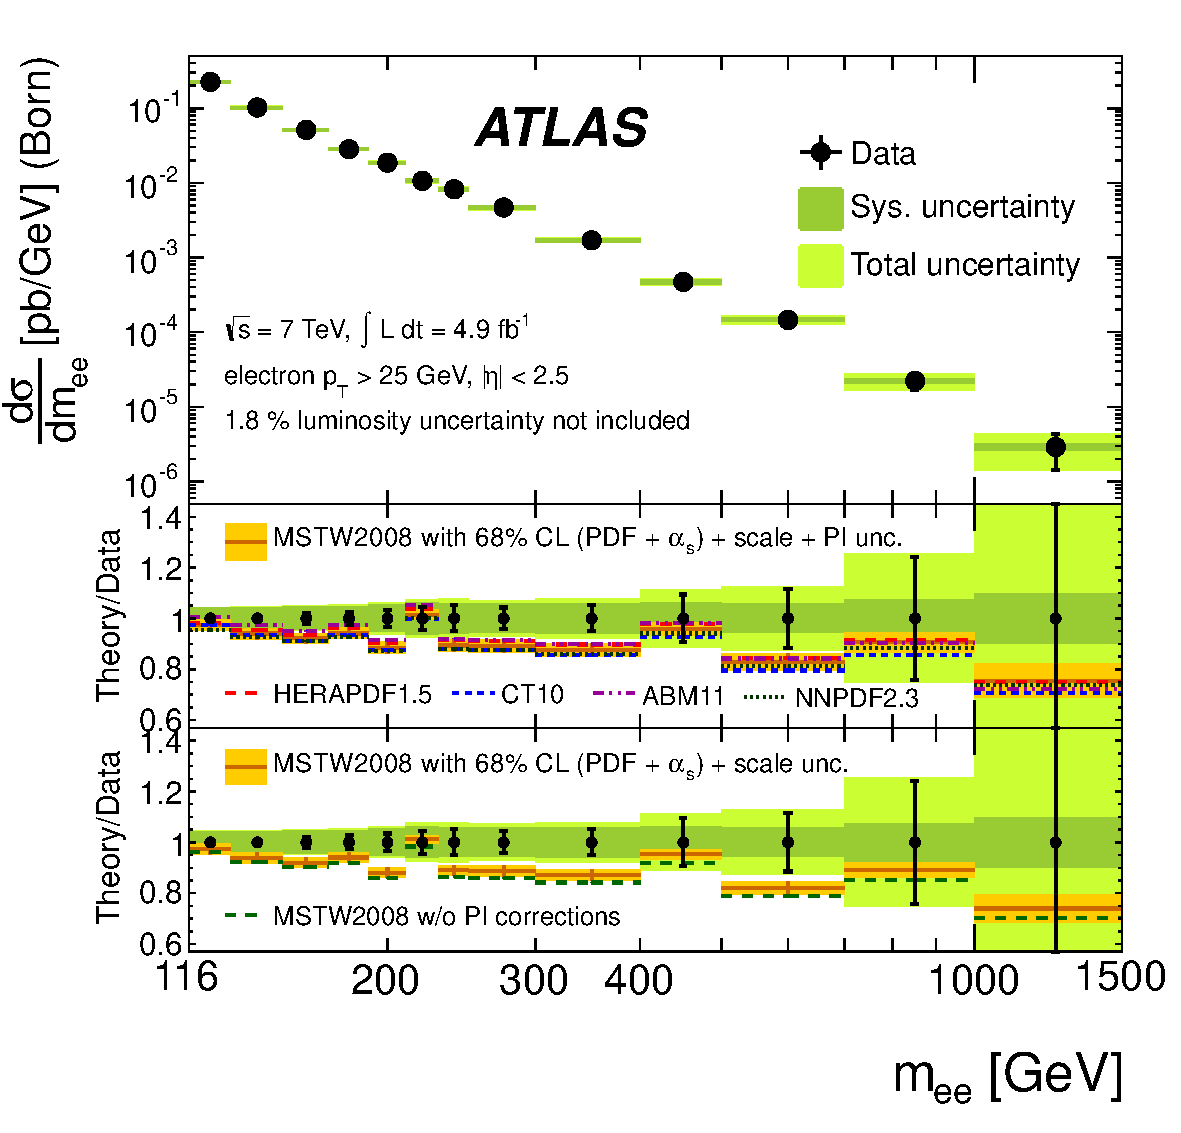
\includegraphics[height=0.3\textheight]{figures/ss-inclboson-drellyan-atlas7tev}
    \caption{Measured differential cross-section at the Born level within the
    fiducial region (electron $\pt > 25 \GeV$ and $|\eta| < 2.5$) with statistical,
     systematic, and combined statistical and systematic (total) uncertainties,
     excluding the 1.8\% uncertainty on the luminosity from ATLAS~\cite{Aad:2013iua}.
     In the upper ratio plot, the photon-induced (PI)
     corrections have been added to the predictions obtained from the MSTW2008,
     HERAPDF1.5, CT10, ABM11 and NNPDF2.3 NNLO PDFs, and for the MSTW2008 prediction
     the total uncertainty band arising from the PDF, $\alpha_s$, renormalisation
     and factorization scale, and photon-induced uncertainties is drawn. The lower
     ratio plot shows the influence of the photon-induced corrections on the
     MSTW2008 prediction, the uncertainty band including only the PDF, $\alpha_s$
     and scale uncertainties.}
    \label{fig:ss-inclboson-drellyan-atlas7tev}
\end{figure}

\begin{figure}[p]
    \centering
    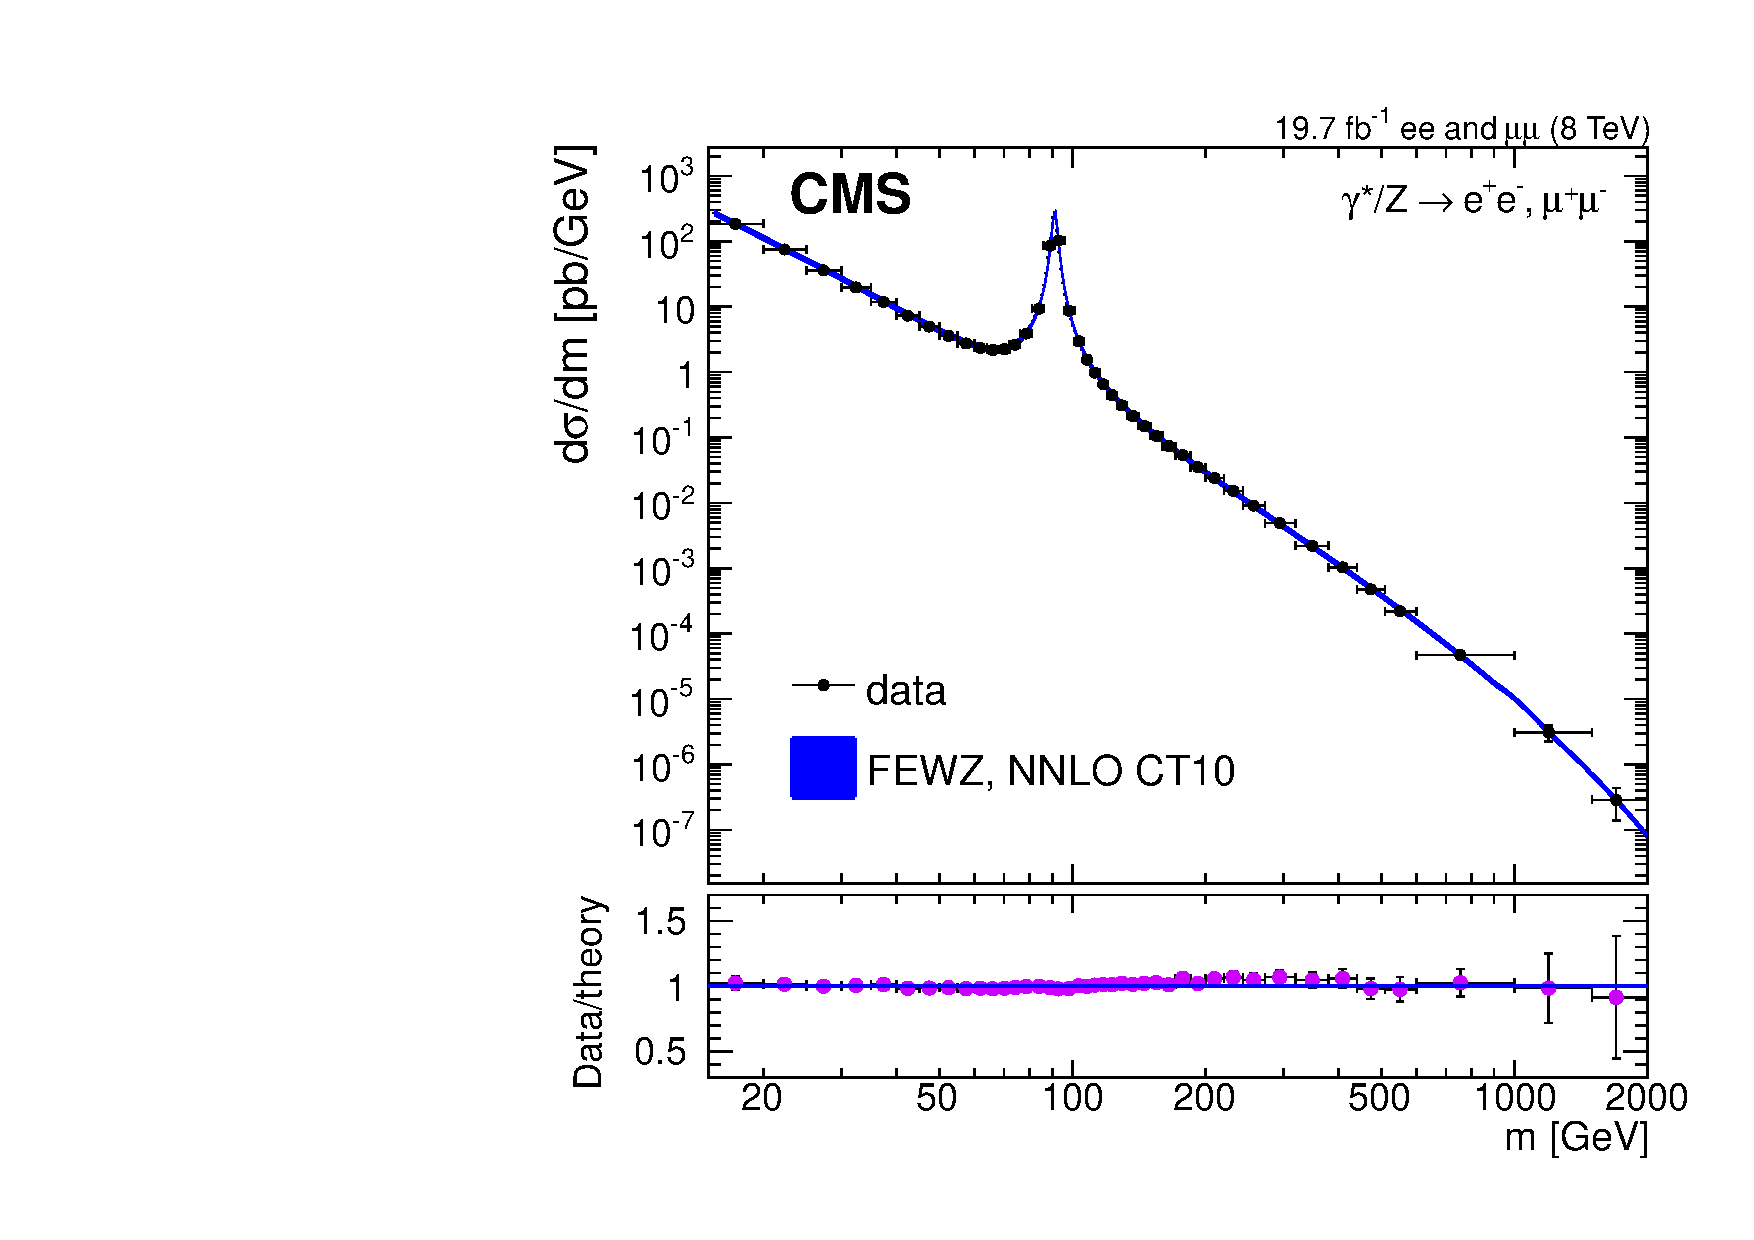
\includegraphics[height=0.3\textheight]{figures/ss-inclboson-drellyan-cms8tev}
    \caption{The DY differential cross section as measured by CMS~\cite{CMS:2014jea} in the combined
dilepton channel and as predicted by NNLO \texttt{FEWZ} 3.1 with CT10 PDF
calculations, for the full phase space.}
    \label{fig:ss-inclboson-drellyan-cms8tev}
\end{figure}

\subsection{Inclusive di-boson production}

ATLAS \Wg \Zg 7 \TeV\xspace~\cite{Aad:2013izg}

CMS \Wg/\Zg 7 \TeV\xspace~\cite{Chatrchyan:2013fya}

CMS $Z(\nu\bar{\nu})\gamma$ 7 \TeV~\cite{Chatrchyan:2013nda}

CMS \Zg 8 \TeV~\cite{Khachatryan:2015kea}


ATLAS simultaneous tt/WW/Z cross section 7 \TeV~\cite{Aad:2014jra}

ATLAS WW 7 \TeV~\cite{ATLAS:2012mec}

ATLAS WW+WZ cross section 7 \TeV~\cite{Aad:2014mda}

ATLAS WW 8 \TeV~\cite{ATLAS-CONF-2014-033}

CMS WW2l2n 7 \TeV~\cite{Chatrchyan:2013yaa}

CMS WWlnjj 7 \TeV~\cite{Chatrchyan:2012bd}

CMS WW/ZZ 8 \TeV~\cite{Chatrchyan:2013oev}

CMS WW2l2n 8 \TeV (CMS-PAS-SMP-14-016, to be published)


ATLAS WZ 7 \TeV~\cite{Aad:2012twa}

CMS VZ 8 \TeV~\cite{Chatrchyan:2014aqa}

CMS WZ at 7+8 \TeV (CMS-PAS-SMP-12-006, to be published)

\subsubsection{ZZ production}
\label{sss-ZZprod}

%short intro
The production of \ZZ in proton-proton collisions has been one of the first di-boson 
processes measured at the LHC. The SM process is and an important and irreducible
background to resonance searches and Higgs production. The production at leading
order is dominated by quark anti-quark annihilation in the $t$ and $u$-channel,
whereas the $s$-channel process is forbidden in the SM 
(see also Figure~\ref{fig:sss-ZZprod-LOdiagrams}). The gluon fusion process 
contributes about 6\% to the total production cross section. 

%FIGURE LO ZZ DIAGRAM
\begin{figure}[htbp]
  \begin{center}
  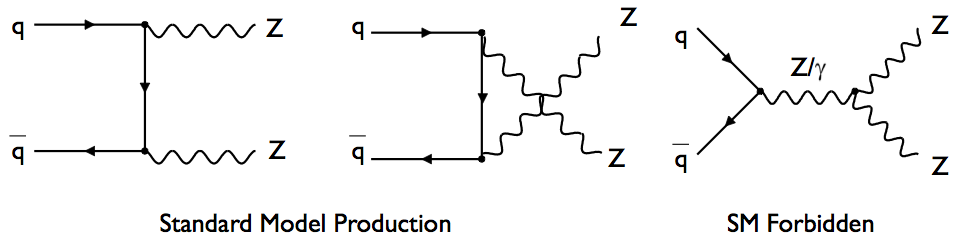
\includegraphics[width=0.9\textwidth]{figures/sss-inclboson-diboson-zzprod-zzdiagram.png}
  \caption{Leading order Feynman diagrams of \ZZ production in the dominant 
  \qqbar\ channel. The \ZZ\ production via the $s$-channel is not allowed in the SM.}
\label{fig:sss-ZZprod-LOdiagrams}
\end{center}
\end{figure}

%decay channels
Precision measurements use the leptonic decay modes of the $Z$ to reduce the impact of
QCD backgrounds. 
The four lepton final state provides an almost background free signature, at the
expense of a relatively small branching ratio 
$BR(ZZ) \to \ll\ll = 0.101^2 \cdot {4 \over 9} = 0.0045$~\cite{PDG}.  
The di-lepton and missing energy channel can exploit the one order of magnitude
higher branching ratio of 
$BR(\ZZ \to \ll\vv) = 0.101 \cdot 0.20 \cdot 2 \cdot {2 \over 3} = 0.0269$, 
at the expense of high background levels.

%analysis CMS and ATLAS.
%ATLAS ZZ 7 TeV~\cite{Aad:2012awa}
%CMS ZZ4l 8 TeV~\cite{Khachatryan:2014dia}
%CMS ZZ4l 7 TeV~\cite{Chatrchyan:2012sga}
%CMS ZZ2l2nu 7+8 TeV~\cite{Khachatryan:2015pba}
The ATLAS collaboration has published results on the $7\TeV$ data-set 
in the $\ll\ll$ and $\ll\vv$ final state~\cite{Aad:2012awa}, and at
$13\TeV$ in the $\ll\ll$ final state~\cite{Aad:2015zqe}. The CMS collaboration
has analysed the full 7 and $8\TeV$ data sets in both 
the $\ll\ll$~\cite{Chatrchyan:2012sga,Khachatryan:2014dia} and 
$\ll\vv$ final state~\cite{Khachatryan:2015pba}.

%Theoretical calculations
% NLO alpha_s arXiv:1105.0020
% NLO alpha_EKW arXiv:1305.5402,arXiv:1307.4331
Theoretical predictions for $\ZZ$ production are available 
at NLO in $\alpha_s$~\cite{arXiv:1105.0020}. In addition, electroweak 
corrections at NLO have been calculated~\cite{arXiv:1305.5402,arXiv:1307.4331}. 

% Z->llll
%Selections
The event selection for the $\ll\ll$ final state requires exactly four leptons 
fulfilling a set of cuts on kinematic quantities. ATLAS and CMS use similar criteria 
as listed in detail in Table~\ref{tab:sss-ZZprod-cuts}. While ATLAS uses $l=e,\mu$,
CMS includes also $\Z\to\tautau$ with subsequent hadronic and leptonic $\tau$
decays. ATLAS uses in addition forward leptons outside the ID tracker
to increase the acceptance by 6\% for electrons and 10\% for muons.
%Backgrounds
The $\ll\ll$ channels offers the cleanest event sample with a background level
of only $2-3\%$ from $\Z+jets$, $\tt$, and di-boson events. 
The background is estimated from data by control regions with looser selection
criteria. 

% Z->llvv
%Selections
Events in the $\ll\vv$ final state are characterized by exactly two leptons 
and missing energy. The event selection requires a leptonic $\Z$ candidate and
missing energy in the event. Both experiments used refined observables of
missing energy with additional information to improve the rejection 
against instrumental background. 
%Backgrounds 
The background level is in the same order
as the signal and substantially higher then for $\ll\ll$ .
Main background sources are $\V+jets$, $\tt$ and di-boson production. 
ATLAS and CMS use data driven techniques to constrain the 
dominant background sources.

% Results at the end?
% xsec
Besides the total cross section for the $pp \to \ZZ$ production process, both
experiments measure also fiducial and differential cross sections. The results are 
summarized in Tabel~\ref{tab:sss-ZZprod-cross-sections}. ATLAS and CMS
use different definitions of the fiducial phase space which needs to be taken into
account to make a direct comparison is possible.
For the total cross section a slightly different mass range for the $\Z$ mass range is
used, where CMS uses a wider range of $60\GeV < \mZ < 120\GeV$ then ATLAS with 
$66\GeV < \mZ < 116\GeV$, which contributes to the difference in the quoted predicted
cross section. Good agreement of experimental and theoretical cross section 
values is observed. 


\begin{table}[htp]
\begin{center}
\resizebox{\textwidth}{!}{
\begin{tabular}{|c|c|c|c|c|c|}
 \hline
 Experiment & decay channel     & \rts & measured $\sigma_{total}$ $[\pb]$                                  & predicted $\sigma_{total}$ $[\pb]$& reference                    \\
 \hline
 ATLAS	     & $\ll\ll$, $\ll\vv$& 7 TeV & {6.7 $\pm$ 0.7 (stat.) $^{+0.4}_{-0.3}$ (syst.) $\pm$ 0.3 (lumi.) }&  6.18$^{+0.25}_{-0.18}$           & \cite{Aad:2012awa}         \\
 CMS	     & $\ll\ll$          & 7 TeV & {6.2 $\pm$ $^{+0.9}_{-0.8}$ (stat.) $^{+0.4}_{-0.3}$ (syst.) $\pm$ 0.1 (lumi.) } & 6.3$\pm 0.4$        & \cite{Chatrchyan:2012sga}  \\
 CMS	     & $\ll\vv$          & 7 TeV & {5.2 $\pm$ $^{+1.5}_{-1.4}$ (stat.) $^{+1.4}_{-1.1}$ (syst.) $\pm$ 0.2 (lumi.) } & 6.1$\pm 0.3$        & \cite{Chatrchyan:2012sga}  \\
 CMS	     & $\ll\ll$          & 8 TeV & {7.7 $\pm$ 0.5 (stat.) $^{+0.5}_{-0.4}$ (syst.) $\pm$ 0.2 (lumi.) } 		        & 7.7$\pm 0.6$        & \cite{CMS:2014xja}         \\ 
 CMS	     & $\ll\vv$          & 8 TeV & {6.9 $\pm$ 0.8 (stat.) $^{+1.8}_{-1.4}$ (syst.) $\pm$ 0.3 (lumi.) }			    & 7.6$\pm 0.3$        & \cite{Chatrchyan:2012sga}  \\% m(ll) > 40GeV, m(vv) > 12GeV
 ATLAS	     & $\ll\ll$			 &13 TeV & {16.7 $\pm$ $^{+2.2}_{-2.0}$ (stat.) $^{+0.9}_{-0.7}$ (syst.) $\pm$ $^{+1.o}_{-0.7}$ (lumi.) }&  15.6$^{+0.4}_{-0.4}$           & \cite{Aad:2015zge}         \\

\hline

\end{tabular}
}
\caption{Summary of measured $\ZZ$ production cross sections from ATLAS and CMS
at 7, 8 and 13 TeV centre-of-mass energies in the four lepton and $\ll\vv$ final state.}
\label{tab:sss-ZZprod-cross-sections}
\end{center}
\label{default}
\end{table}%


%%%%
% THIS MIGHT GO INTO THE SECTION ON TGC
% aTGC
% Spectra ATGC
% charged pT : llvv CMS
% m(llll) : llll CMS
% pT(Z) : llll,llvv ATLAS
Limits on ATGC parameters are determined with differential distributions of the 
invariant di-boson mass (CMS, four lepton channel), 
the transverse momentum of the leading lepton (CMS, $\ll\vv$-channel), or
the transverse momentum of the leading \Z (ATLAS, all channels).
A comparison of the measured and predicted differential cross sections in the 
four-lepton invariant mass is shown from CMS in Figure \ref{fig:sss-inclboson-diboson-zzprod-zzinvmass}.
Also shown is the prediction in the presence of a non-zero value of the anomalous coupling
parameter $f_4^Z=0.015$, which shows an enhancement over the SM value at high 
invariant masses. 

%FIGURE ZZ invariant mass
%1406.0113v2.pdf, FIGURE 5
% https://twiki.cern.ch/twiki/pub/CMSPublic/PhysicsResultsSMP13005/fig5tgcA.pdf
% CMS ZZ 4l 8 TeV
\begin{figure}[htbp]
  \begin{center}
  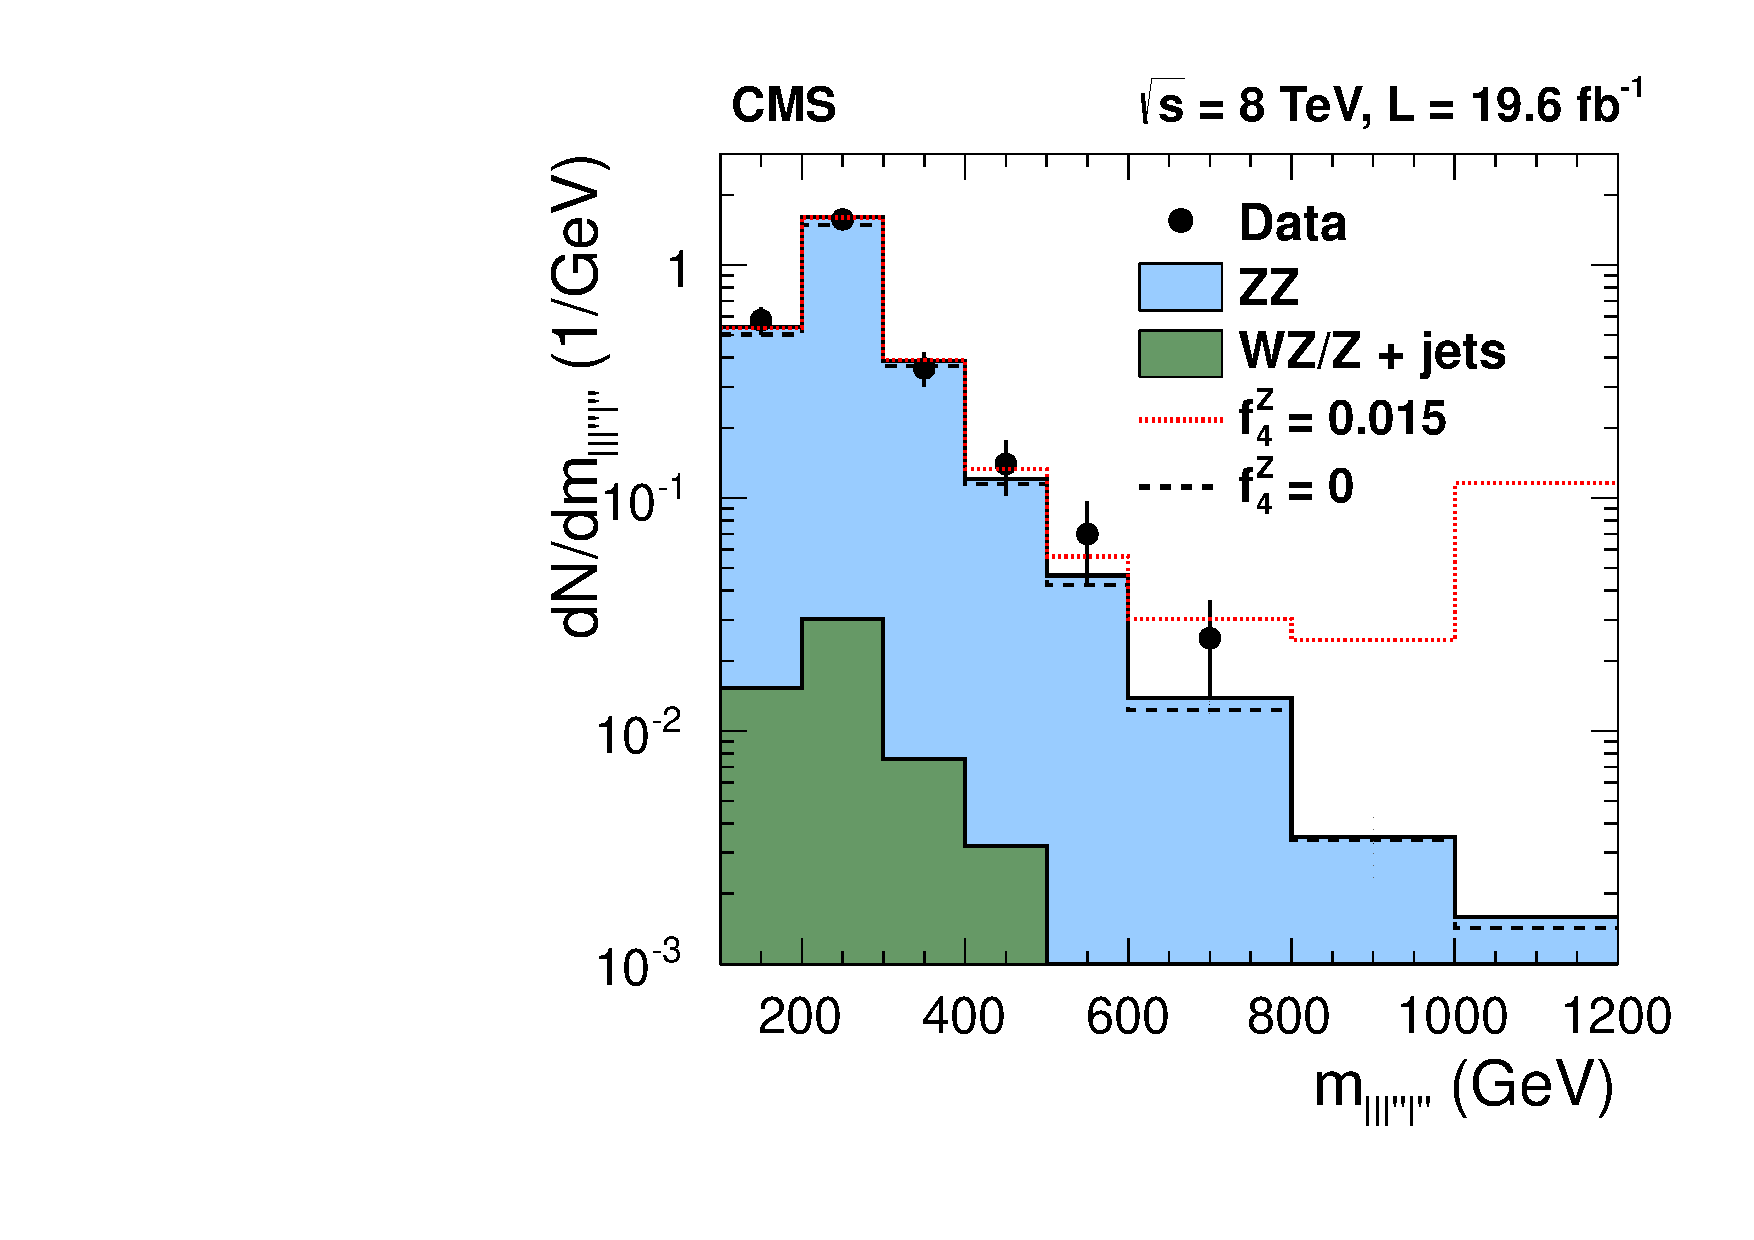
\includegraphics[width=0.9\textwidth]{figures/sss-inclboson-diboson-zzprod-zzinvmass.pdf}
  \caption{ Distribution of the four-lepton reconstructed mass for the combined $4e$, $4\mu$, and $2e2\mu$ channels from CMS~\cite{Khachatryan:2014dia}. Points represent the data, the shaded histogram labeled $\ZZ$ represents the predictions for $\ZZ$ signal, the histograms labeled $\WZ$/$\Z$+jets shows background estimated form data. The dashed and dotted histograms indicate the SM expectation (f4Z = 0) and in the presence of an ATGC (f4Z = 0.015) with all the other anomalous couplings set to zero. The last bin includes all entries with masses above 1000 GeV.
}
\label{fig:sss-inclboson-diboson-zzprod-zzinvmass}
\end{center}
\end{figure}

Both experiment publish 95\% CL limits on ATGC without form factors in the $\ll\ll$ 
and $\ll\vv$ channels. The results are in agreement with the SM and 
summarized in Figure~\ref{fig:sss-inclboson-diboson-zzprod-aTGC_naTGCf} 
taken from Ref. \cite{aTGCplots}. The precision of the LHC results is driven by the steep increase of 
sensitivity with higher centre-of-mass energy
and are about 2 orders of magnitude better compared to the 
combined LEP result~\cite{LEP-comb-2002}.  
% FIGURE COMPARISON OF ZZ NTGC
% https://twiki.cern.ch/twiki/bin/view/CMSPublic/PhysicsResultsSMPaTGC
% M Herndon
% FETCHED 34RD JULY 2015
\begin{figure}[htbp]
  \begin{center}
  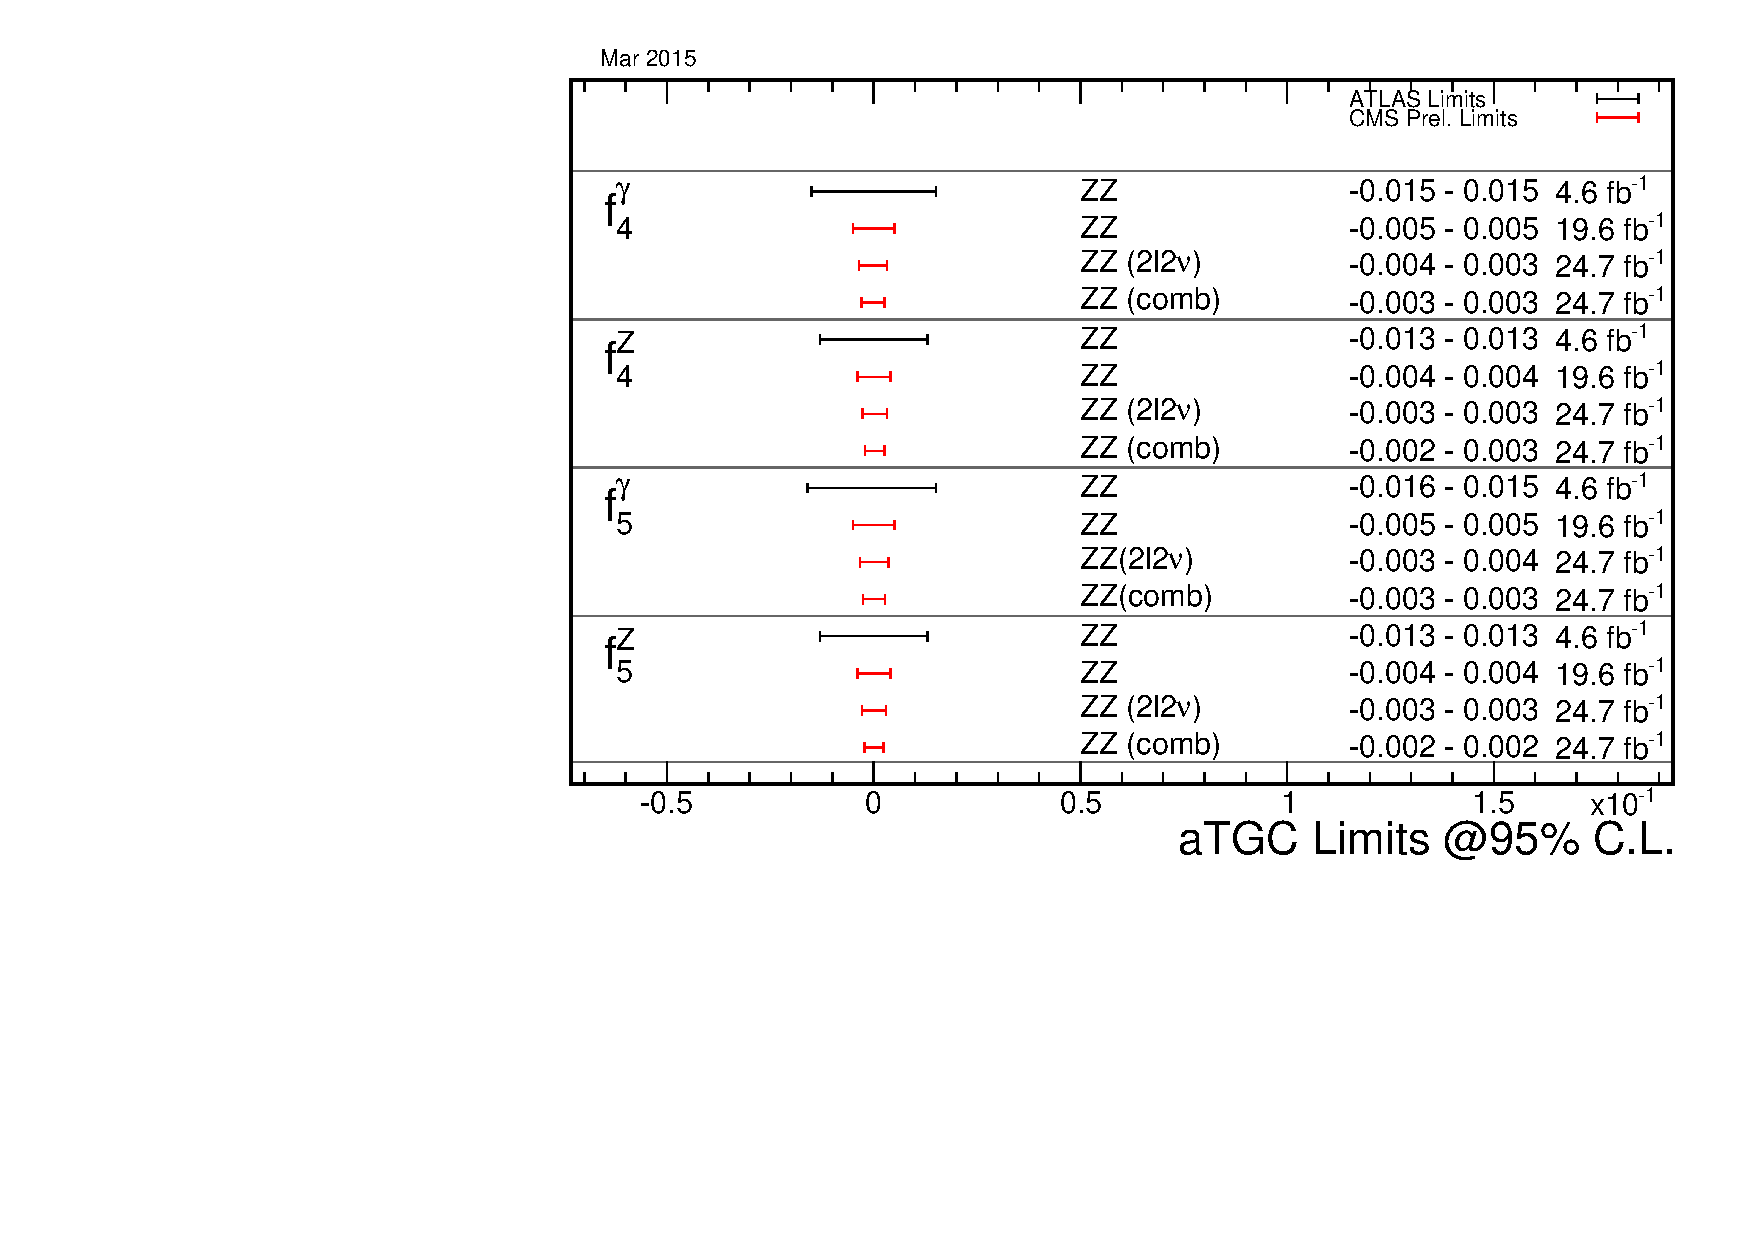
\includegraphics[width=0.9\textwidth]{figures/sss-inclboson-diboson-zzprod-aTGC_naTGCf.pdf}
  \caption{ Comparison of the limits on \ffourv{} and \ffivev{} from ATLAS and CMS in the $\ll\ll$ and $\ll\vv$
  channel at 7 and $8\TeV$.}
\label{fig:sss-inclboson-diboson-zzprod-aTGC_naTGCf}
\end{center}
\end{figure}








%ATLAS ZZ 7 TeV~\cite{Aad:2012awa}
%CMS ZZ4l 8 TeV~\cite{Khachatryan:2014dia}
%CMS ZZ4l 7 TeV~\cite{Chatrchyan:2012sga}
%CMS ZZ2l2nu 7+8 TeV~\cite{Khachatryan:2015pba}

\subsubsection{WZ production}

\label{sss-WZprod}

%short intro
At the LHC, \WZ\ diboson are produced from quark-antiquark initial states at 
leading order (LO) and quark-gluon initial states at next-to-leading order 
(NLO). %~\cite{PhysRevD.65.094041}
%Figure~\ref{fig:LOdiagrams} shows the LO Feynman diagrams for \WZ production from $q\bar{q}'$ initial states. 
The SM allowed $s$-channel diagram has a triple boson vertex and is sensitive to 
ATGC.

%FIGURE LO WZ DIAGRAM
% may include 
% figures/sss-inclboson-diboson-wzprod-wz-s-channel.pdf
% figures/sss-inclboson-diboson-wzprod-wz-t-channel.pdf
% figures/sss-inclboson-diboson-wzprod-wz-u-channel.pdf

%\begin{figure}[htbp]
%  \begin{center}
%  \includegraphics[width=0.9\textwidth]{figures/sss-inclboson-diboson-wzprod-wzdiagram.png}
%  \caption{Leading order Feynman diagrams of \WZ production in the dominant 
%  \qqbar\ channel.}
%\label{fig:sss-WZprod-LOdiagrams}
%\end{center}
%\end{figure}

%decay channels


%analysis CMS and ATLAS.
%ATLAS WZ 8 TEV \cite{Aad:2016ett} 
%ATLAS WZ 7 \TeV~\cite{Aad:2012twa}
% - figure from https://atlas.web.cern.ch/Atlas/GROUPS/PHYSICS/PAPERS/STDM-2012-09/
%CMS WZ at 7+8 \TeV (CMS-PAS-SMP-12-006, to be published)
The ATLAS experiment measured the \WZ\ production cross section in the fully 
leptonic decay channel \ll\lnu\; at $\rts = 7\TeV$~\cite{Aad:2012twa} and $\rts = 8\TeV$~\cite{Aad:2016ett} 
and set limits on charged ATGC.
%Theoretical calculations
% TBD
% WZ->lllv
%Selections
In these analyses the final states involving electrons or muons are considered signal,
whereas boson decays to tau's are considered as background.  
%Backgrounds
The dominant background sources are \Zboson+jet and \ZZ production, accounting for about 40\% of 
the overall background. The overall signal over background ratio is about $4$.
%systematics
The leading systematic uncertainty is related to the data-driven estimation method of the   
background.%, with the dominant Z + jets contributing ($\pm3.8\%$).

% Results at the end
% xsec
The fiducial cross section for the 7 TeV (8 TeV) analysis is defined by $\pt^{\mu,e} > 15\GeV$ for the leptons from the \Zboson\ 
 decay, $\pt^{\mu,e} > 20\GeV$ for the lepton from the \Wboson, $|\eta^{\mu,e}|<2.5$, $\pt^\nu>25\GeV$,
 $|m_ll-m_Z| < 10(25)\GeV$, $M_T^W>20(30)GeV$ and $\Delta R> 0.3$ for the three possible $\ell\ell$ pairings. 
The total cross section requires the mass of the \Zboson\ to be in the range of $66\GeV < |m_Z| < 116\GeV$
to suppress the contribution from $\gamma^*$.
The fiducial and total cross sections are compared to the SM expectation at NLO in Table~\ref{tab:sss-WZprod-xsec}.

\begin{table}[htp]
\begin{center}
\resizebox{\textwidth}{!}{
\begin{tabular}{|c|c|c|c|c|c|}
Experiment & cross section & \rts & measured  & predicted  & reference  \\ \hline
ATLAS & total & 7 GeV & {19$^{+1.4}_{-1.3}$ (stat.) $\pm{0.9}$ (syst.) $\pm$ 0.4 (lumi.) pb}  & {17.6 $^{+1.1}_{-1.0}$ pb} & \cite{Aad:2012twa} \\
ATLAS & total & 8 GeV & {24.3$\pm 0.6$ (stat.) $\pm{0.6}$ (syst.) $\pm{0.4}$ (theo.) $\pm$ 0.5 (lumi.) pb}  & {21.0  $\pm$ 1.6 pb} & \cite{Aad:2016ett} \\
ATLAS & fiducial & 7 GeV & {92 $\pm$ $^{+7}_{-6}$ (stat.) $\pm{4}$ (syst.) $\pm$ 2 (lumi.) fb}  & -- & \cite{Aad:2012twa} \\
ATLAS & fiducial & 8 GeV & {35 $\pm$ $\pm{0.9}$ (stat.) $\pm{0.8}$ (syst.) $\pm$ 0.8 (lumi.) fb}  & {30 $\pm$ $\pm{0.5}$ (PDF) $\pm{0.8}$ (scale) fb} & \cite{Aad:2016ett} \\
\end{tabular}
}
\caption{Summary of measured fiducial and total $\WZ$ production cross sections from ATLAS 
at 7 TeV centre-of-mass energies in the $\ll\lnu$ final state. The fiducial definitions differ from the 7 and 8 TeV analysis. Further, the 7 TeV analysis
quotes the sum for the $e$ and $\mu$ channels, the 8 TeV analysis quotes the combination of channels. Thus, the two fiducial cross sections cannot be 
compared directly.}
\end{center}
\label{tab:sss-WZprod-xsec}
\end{table}%


% unfolded spectra
In Figure~\ref{fig:sss-WZprod-ptZ-det} the differential cross section measured in bins of 
$\pt^Z$ is shown, compared to SM prediction and a set of anomalous TGC couplings. 
The normalized $\pt^Z$ spectrum is unfolded and compared to the NLO calculation of \mcatnlo in 
Figure~\ref{fig:sss-WZprod-ptZ-det}, showing good agreement with the SM.


\begin{figure}[htbp]
  \begin{center}
  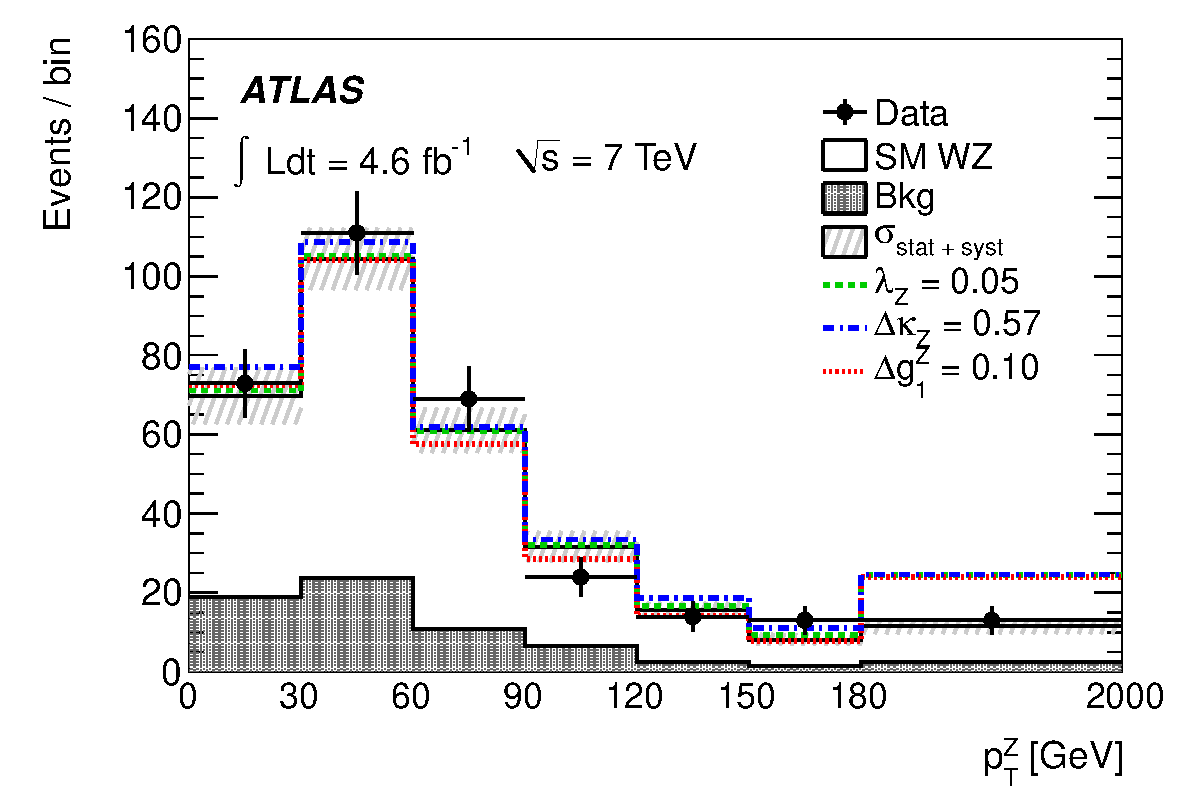
\includegraphics[width=0.45\textwidth]{figures/sss-inclboson-diboson-wzprod-ptZ-det.pdf}
  \caption{ATLAS measurement of the transverse momentum of the \Zboson in \WZ events ($\pt^Z$) compared with the SM prediction at $\rts = 7\TeV$. For illustration calculations for a set of anomalous couplings values are also shown. The full uncertainty contains statistical and systematic uncertainties.}
\label{fig:sss-WZprod-ptZ}
\end{center}
\end{figure}

\begin{figure}[htbp]
  \begin{center}
  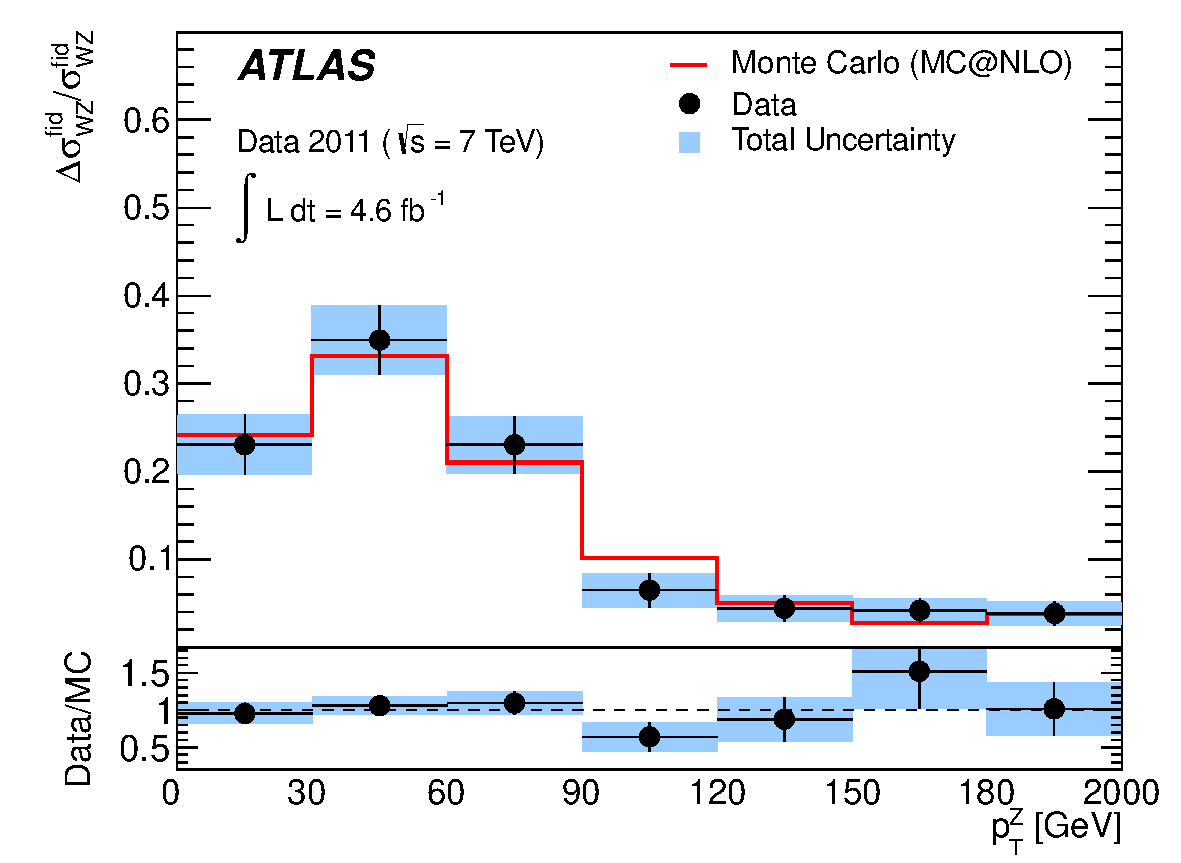
\includegraphics[width=0.45\textwidth]{figures/sss-inclboson-diboson-wzprod-ptZ.pdf}
  \caption{ATLAS measurement of the normalized fiducial cross-sections in bins of $\pt^Z$ compared with the SM prediction at $\rts = 7\TeV$. The full uncertainty contains statistical and systematic uncertainties.}
\label{fig:sss-WZprod-ptZ-det}
\end{center}
\end{figure}


%%%%
% THIS MIGHT GO INTO THE SECTION ON TGC
% aTGC
Limits on the charged ATGC parameters \dkz, \lz\ and \gz\ are extracted from the transverse momentum distribution
of the \Zboson, $\pt^Z$~\cite{Aad:2012twa} or from the transverse mass of the $\Wboson\Zboson$ system~\cite{Aad:2016ett}. 
The ATGC parameter 95\% CL limits using a dipole form-factor with a cut-off of $\Lambda=2\TeV$ and without a form-factor are quoted 
in Table~\ref{tab:sss-WZprod-ATGC} from the more constraining $8\TeV$ data set analysis~\cite{Aad:2016ett}.

%\begin{table}\centering
%\caption{Expected and observed 95\% CL on 
%\dkz, \lz\ and \gz.}
%\label{tab:sss-WZprod-ATGC}
%\begin{tabular}{ccccc}
%\hline
%& $\rts$,  & Observed & Observed & Expected \\
%& & $\Lambda=2$~TeV & no form factor & no form factor\\
%\hline
%$7\TeV$ & $\gz$ & $[-0.074, 0.133]$ & $[-0.057, 0.093]$ & $[-0.046, 0.080]$ \\
%$7\TeV$ & $\dkz$ & $[-0.42, 0.69]$ & $[-0.37, 0.57]$ & $[-0.33, 0.47]$ \\
%$7\TeV$ & $\lz$ & $[-0.064, 0.066]$ & $[-0.046, 0.047]$ & $[-0.041, 0.040]$ \\
%\hline
%\end{tabular}
%\end{table}


\begin{table}\centering 
\begin{tabular}{cccc}
\hline
 $\Lambda$ & Coupling & Expected  & Observed \\
\hline
2 TeV 	& $\gz$ 		& [$-0.023$, $0.055$]  & [ $-0.029$, $0.050$] \\ \\
2 TeV 	& $\dkz$ 	& [$-0.17$, $0.25$]    & [$-0.19$, $0.30$] \\
2 TeV 	& $\lz$ 	& [$-0.016$, $0.016$]  & [$-0.016$, $0.016$] \\
\hline
\end{tabular}
\caption{Expected and observed 95\% CL on \dkz, \lz\ and \gz\; for a cut-off parameter $\Lambda = 2\TeV$ and $\Lambda = \infty$.}
 \label{tab:sss-WZprod-ATGC}
\end{table}
 

% WZ->llqq ????











\subsubsection{WW production}
\label{sss-WWprod}

%short intro
The \WW\ production process has the highest production cross section
among the massive vector di-boson processes. It is also an important
background process to Higgs production and to searches for new physics.
%analysis CMS and ATLAS.
%    ** ATLAS (5.6ifb, 7TeV, TGC), Phys. Rev. D 87, 112001 (2013), http://arxiv.org/abs/1210.2979
%	    ATLAS (20ifb 8TeV), https://atlas.web.cern.ch/Atlas/GROUPS/PHYSICS/CONFNOTES/ATLAS-CONF-2014-033/ 
%    ** CMS (7 TeV, 5 fb-1, TGC)  WW cross section in the lvlv channel at 7 TeV  http://arxiv.org/abs/1306.1126
%    ** CMS (8 TeV, 3.5 fb-1 WW, 5.3 fb-1 ZZ) , Phys. Lett. B 721 (2013) 190, WW and ZZ at 8 TeV, http://arxiv.org/abs/1301.4698 
%	    CMS (20ifb, 8TeV), submitted to EPJC,  http://arxiv.org/abs/1507.03268
ATLAS and CMS, observed the \WW\ production process in 
the fully leptonic channel and published results for 7 TeV 
(ATLAS~\cite{ATLAS:2012mec}, CMS~\cite{Chatrchyan:2013yaa}) and
8 TeV (CMS~\cite{Chatrchyan:2013oev}) center-of-mass energy. 
%decay channels
Three final states, namely $ee$, $\mu\mu$, and $e\mu$ are included in the analyses. 
The contribution from leptonically decaying $\tau$ leptons is included in the signal
definition. Although the production cross section is relatively high, the signature of two opposite 
sign leptons and missing transverse energy is shared with many processes and a careful
control of the backgrounds is necessary to achieve a precise measurement.

%Theoretical calculations
% TBD -> General section about theoretical calculations?

%Selections
Candidate $\WW$ events are selected by requiring two oppositely-charged leptons 
accompanied with large \MET. 
%Backgrounds
The dominant background sources are \ttbar\; and single top quark, 
$\W/$+jets, followed by $\Zzero/\gamma^{*}$+jets production.
To suppress the dominant \ttbar\; background, events with one or more jets are rejected.   
Additional requirements on \MET\ and the use of top quark-taggers further reduce the residual background
%ATLAS: 685 WW, 275 background => b / (s+b) = 29%
%CMS: 824WW, 369 background => b / (s+b) = 31%
to about 30\%.  
%systematics
The dominant systematic uncertainty is related to the jet veto efficiency 
and estimated to be about 5\% for the \WW\, production. 
The experiments quote a theoretical uncertainty on the signal acceptance due to 
variations of the parton distribution functions and renormalization and factorization 
scales in the range of 1-2\%.

% Results at the end
% total xsec
% ATLAS 7TeV 4.6 ifb: xsec(WW) = 51.9 +- 2.0 (stat) +- 3.9 (sys) +- 2.0 (lum) pb
%                     xsec_theo(WW) = 44.7 +2.1 -1.9 pb
% CMS 7TeV 4.9 ifb: xsec(ww) = 52.4 +- 2.0 (stat) +- 4.5 (syst) +- 1.2 (lum) pb
%                   xsec_theo(WW) = 47.0 +- 2.0 pb
% CMS 8TeV 5ifb: xsec(WW) = 69.9 +- 2.8 (stat) +- 5.6 (sys) +- 3.1 (lum) pb
%                xsec_theo(WW) = 57.3 +2.3 -1.6 pb (not including H ~ 4%)

% definition of total xsecs might differ (inclusion of higgs or not).
Both ATLAS and CMS provide a measurement of the total cross section for the process $pp \rightarrow \WW$
and compare to theoretical calculations. The Higgs process contributes with about 4\% to the total 
cross section and has not been taken into account in the comparison to the SM predictions.
The total cross section results are summarized in Table~\ref{tab:sss-WWprod-xsec}.
A good agreement between the experiments for the measured cross section as well as for the theoretical predictions
is observed.
% fiducial xsec
A normalized differential measurement of the fiducial cross section in bins of $\pt$ of the leading lepton is presented by ATLAS,
as shown in Figure~\ref{fig:sss-WWprod-pt-fiducial}. The unfolded spectrum is in agreement with the SM prediction.

\begin{table}[htp]

\begin{center}
\resizebox{\textwidth}{!}{
\begin{tabular}{|c|c|c|c|c|c|}
Experiment & cross section & \rts\; [TeV] & measured [pb]  & predicted [pb] & reference  \\ \hline
ATLAS & total & 7 & {51.9 $\pm 2.0$  (stat.) $\pm$ ${3.9}$ (syst.) $\pm$ 2.0 (lumi.) }  & {44.7 $^{+2.1}_{-1.9}$ } & \cite{ATLAS:2012mec} \\
CMS & total & 7 & {52.4 $\pm 2.0$  (stat.) $\pm$ ${4.5}$ (syst.) $\pm$ 1.2 (lumi.) }  & {47.0 $\pm 2.0$ } & \cite{Chatrchyan:2013yaa} \\
CMS & total & 8 & {69.9 $\pm 2.8$  (stat.) $\pm$ ${5.6}$ (syst.) $\pm$ 3.1 (lumi.) }  & {57.3 $^{+2.3}_{-1.6}$} & \cite{Chatrchyan:2013yaa} \\
\end{tabular}
}
\caption{Summary of measured fiducial and total $\WW$ production cross sections from ATLAS and CMS 
at 7 and 8 TeV center-of-mass energies in the $\lnu\lnu$ final state.}
\end{center}
\label{tab:sss-WWprod-xsec}
\end{table}%

% unfolded spectra
% https://atlas.web.cern.ch/Atlas/GROUPS/PHYSICS/PAPERS/STDM-2012-01/fig_07.pdf
% 
\begin{figure}[htbp]
  \begin{center}
  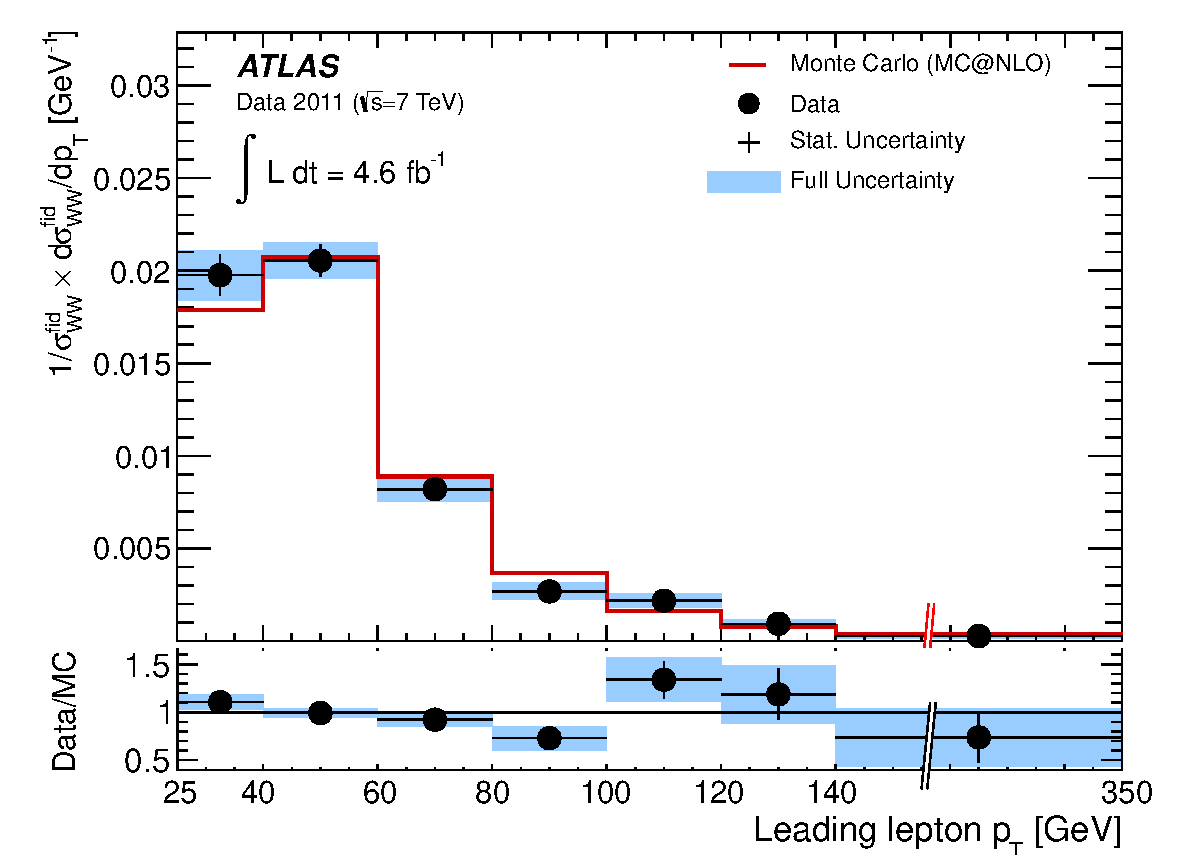
\includegraphics[width=0.45\textwidth]{figures/sss-inclboson-diboson-wwprod-pt-fiducial.pdf}
  \caption{ATLAS measurement~\cite{ATLAS:2012mec} of the transverse momentum of the leading lepton in \WW events compared with the SM prediction at $\rts = 7\TeV$. The full uncertainty contains statistical and systematic uncertainties.}
\label{fig:sss-WWprod-pt-fiducial}
\end{center}
\end{figure}


%%%%
% THIS MIGHT GO INTO THE SECTION ON TGC
% aTGC
The leading lepton $\pt$ spectrum of the \WW process is sensitive to anomalous gauge boson coupling parameters
\dkg,  \dkz, \lg, \lz, and \dgz. Both ATLAS and CMS quote limits in the LEP 
parametrization~\cite{Gounaris:1996rz} that introduces $SU(2) \times U(1)$ gauge invariance 
constraints to reduce the number of free parameters to \dgz,  \dkg, and \lz. The obtained limits assuming 
no form factor are compared for both expected and measured 95\% CL limits in Table~\ref{tab:sss-WZprod-ATGC}.

\begin{table}\centering
\begin{tabular}{cccc}
\hline
& Observed (CMS) & Observed (ATLAS) & Expected (ATLAS)\\
\hline
$\dgz$ & $[-0.095, 0.095]$ & $[-0.039, 0.052]$ & $[-0.039, 0.052]$ \\
$\dkg$ & $[-0.21, 0.22]$ & $[-0.14, 0.14 ]$ & $[-0.13, 0.13]$ \\
% ATLAS DKZ limits converted to DKG with DKG = c2/s2(DG1-DKZ) = 3.3252 * (-DKZ) [DG1 == 0]
$\lz$ & $[-0.048, 0.048]$ & $[-0.062, 0.059]$ & $[-0.060, 0.059]$ \\
\hline
\end{tabular}
\caption{Expected and observed 95\% CL limits on the ATGC parameters 
\dkg, \lz\ and \dgz\; in the LEP parametrization derived from the leading lepton $\pt$ spectrum in \WW production at 7 TeV (ATLAS~\cite{ATLAS:2012mec}, CMS~\cite{Chatrchyan:2013yaa}). No form-factor is applied to the ATGC parameters.}
\label{tab:sss-WZprod-ATGC}
\end{table}










\subsection{Inclusive tri-boson production}

One avenue for testing quartic gauge boson interactions is through
inclusive tri-boson production: $pp\ to VV^{\prime}V^{\prime\prime}$
for $V= \gamma, W, Z$.  Using the Run 1 data sample, the triply heavy
such channels ($WWW, WWZ, WZZ, ZZZ$) are not accessible anywhere near
SM rates, due to their small 8 TeV cross sections and large
multi-lepton backgrounds. The photonic channels do not suffer as much
from these problems, and sensitivity is at or near SM rates in Run 1. 

ATLAS $W\gamma\gamma$~\cite{Aad:2015uqa}
\begin{figure}[p]
    \centering
    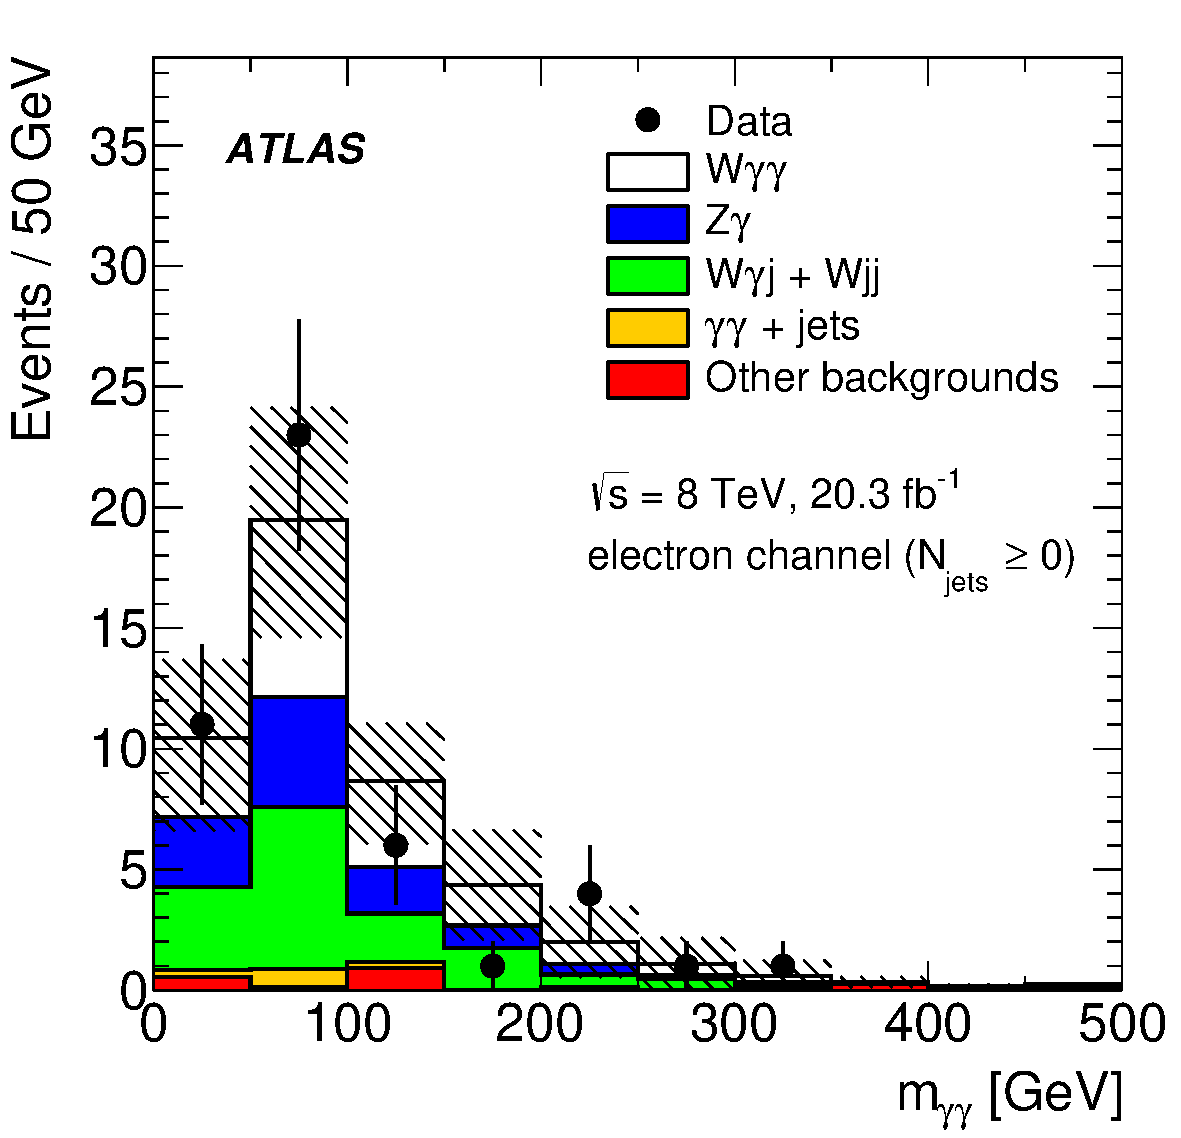
\includegraphics[width=0.45\textwidth]{figures/ss-inclboson-triboson-wgg-ele-atlas8tev.pdf}
    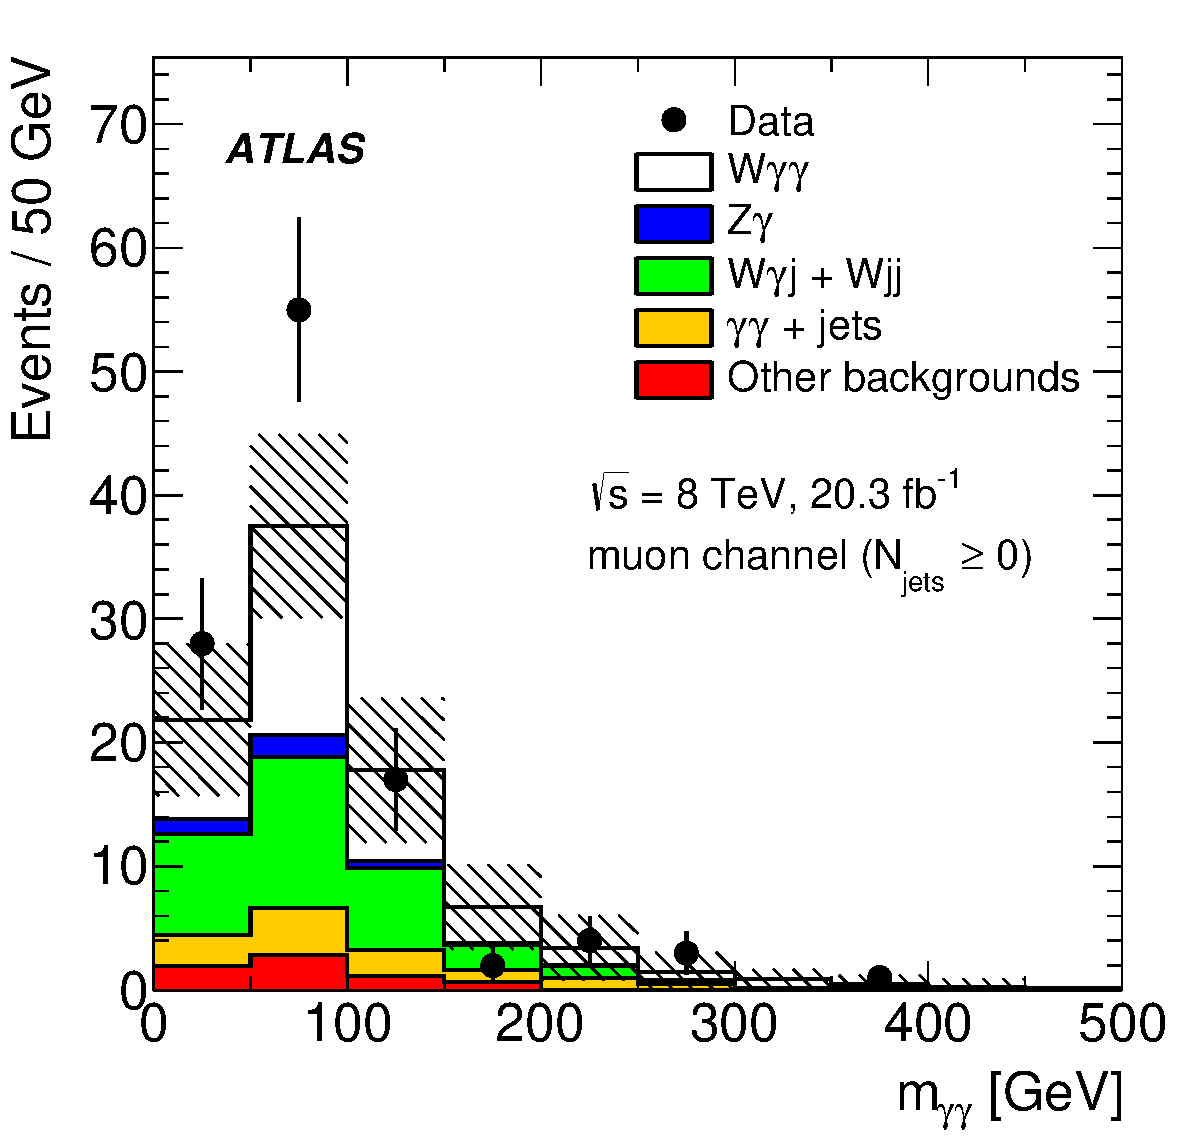
\includegraphics[width=0.45\textwidth]{figures/ss-inclboson-triboson-wgg-mu-atlas8tev.pdf}
    \caption{}
    \label{fig:ss-inclboson-triboson-wgg-atlas8tev}
\end{figure}


CMS WVgamma 8 \TeV~\cite{Chatrchyan:2014bza}

\begin{figure}[p]
    \centering
    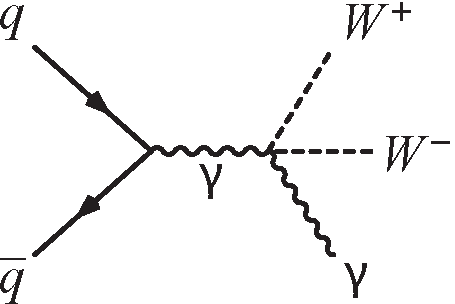
\includegraphics[width=0.45\textwidth]{figures/ss-inclboson-triboson-wvg-diagram1.pdf}
    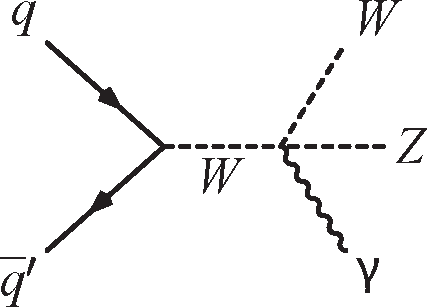
\includegraphics[width=0.45\textwidth]{figures/ss-inclboson-triboson-wvg-diagram2.pdf}
    \caption{}
    \label{fig:ss-inclboson-triboson-wvg-diagrams}
\end{figure}
\begin{figure}[p]
    \centering
    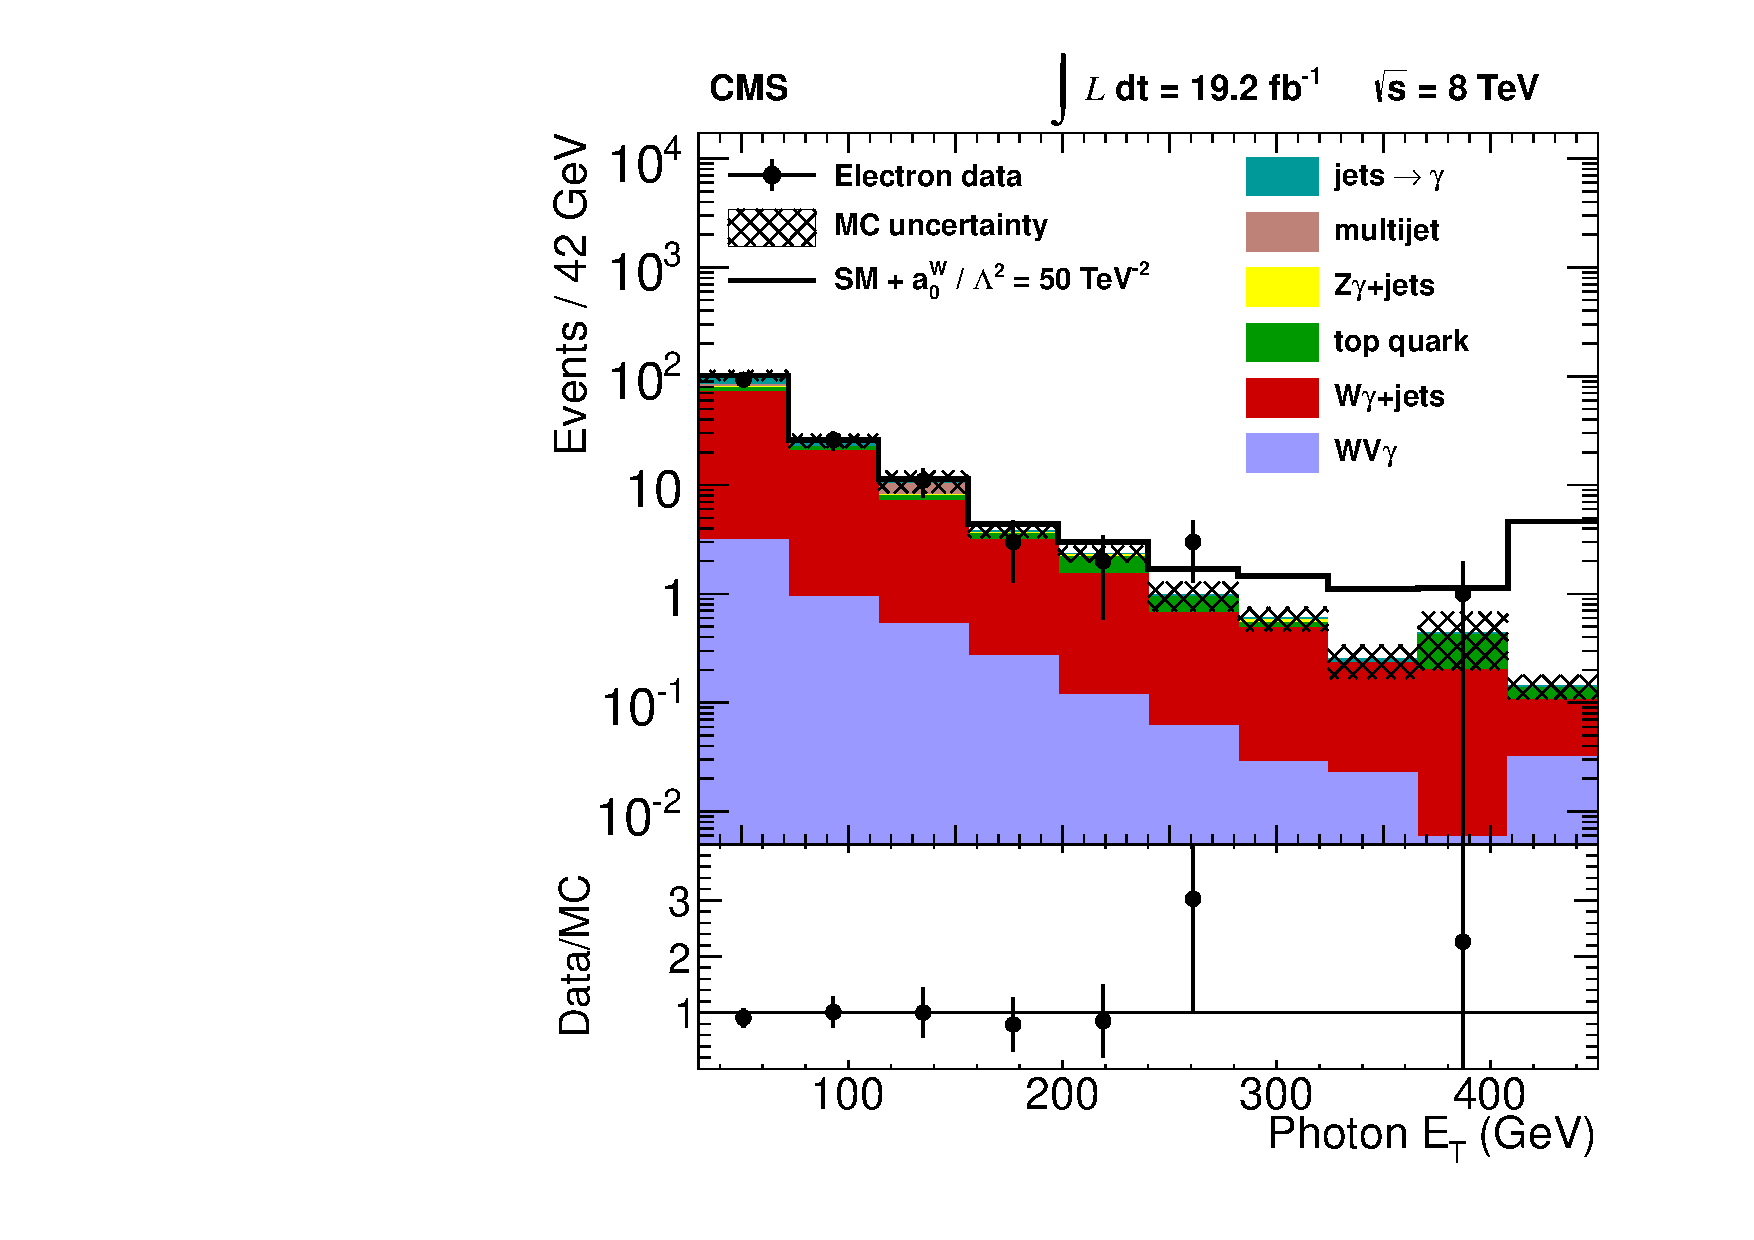
\includegraphics[width=0.45\textwidth]{figures/ss-inclboson-triboson-wvg-ele-cms8tev.pdf}
    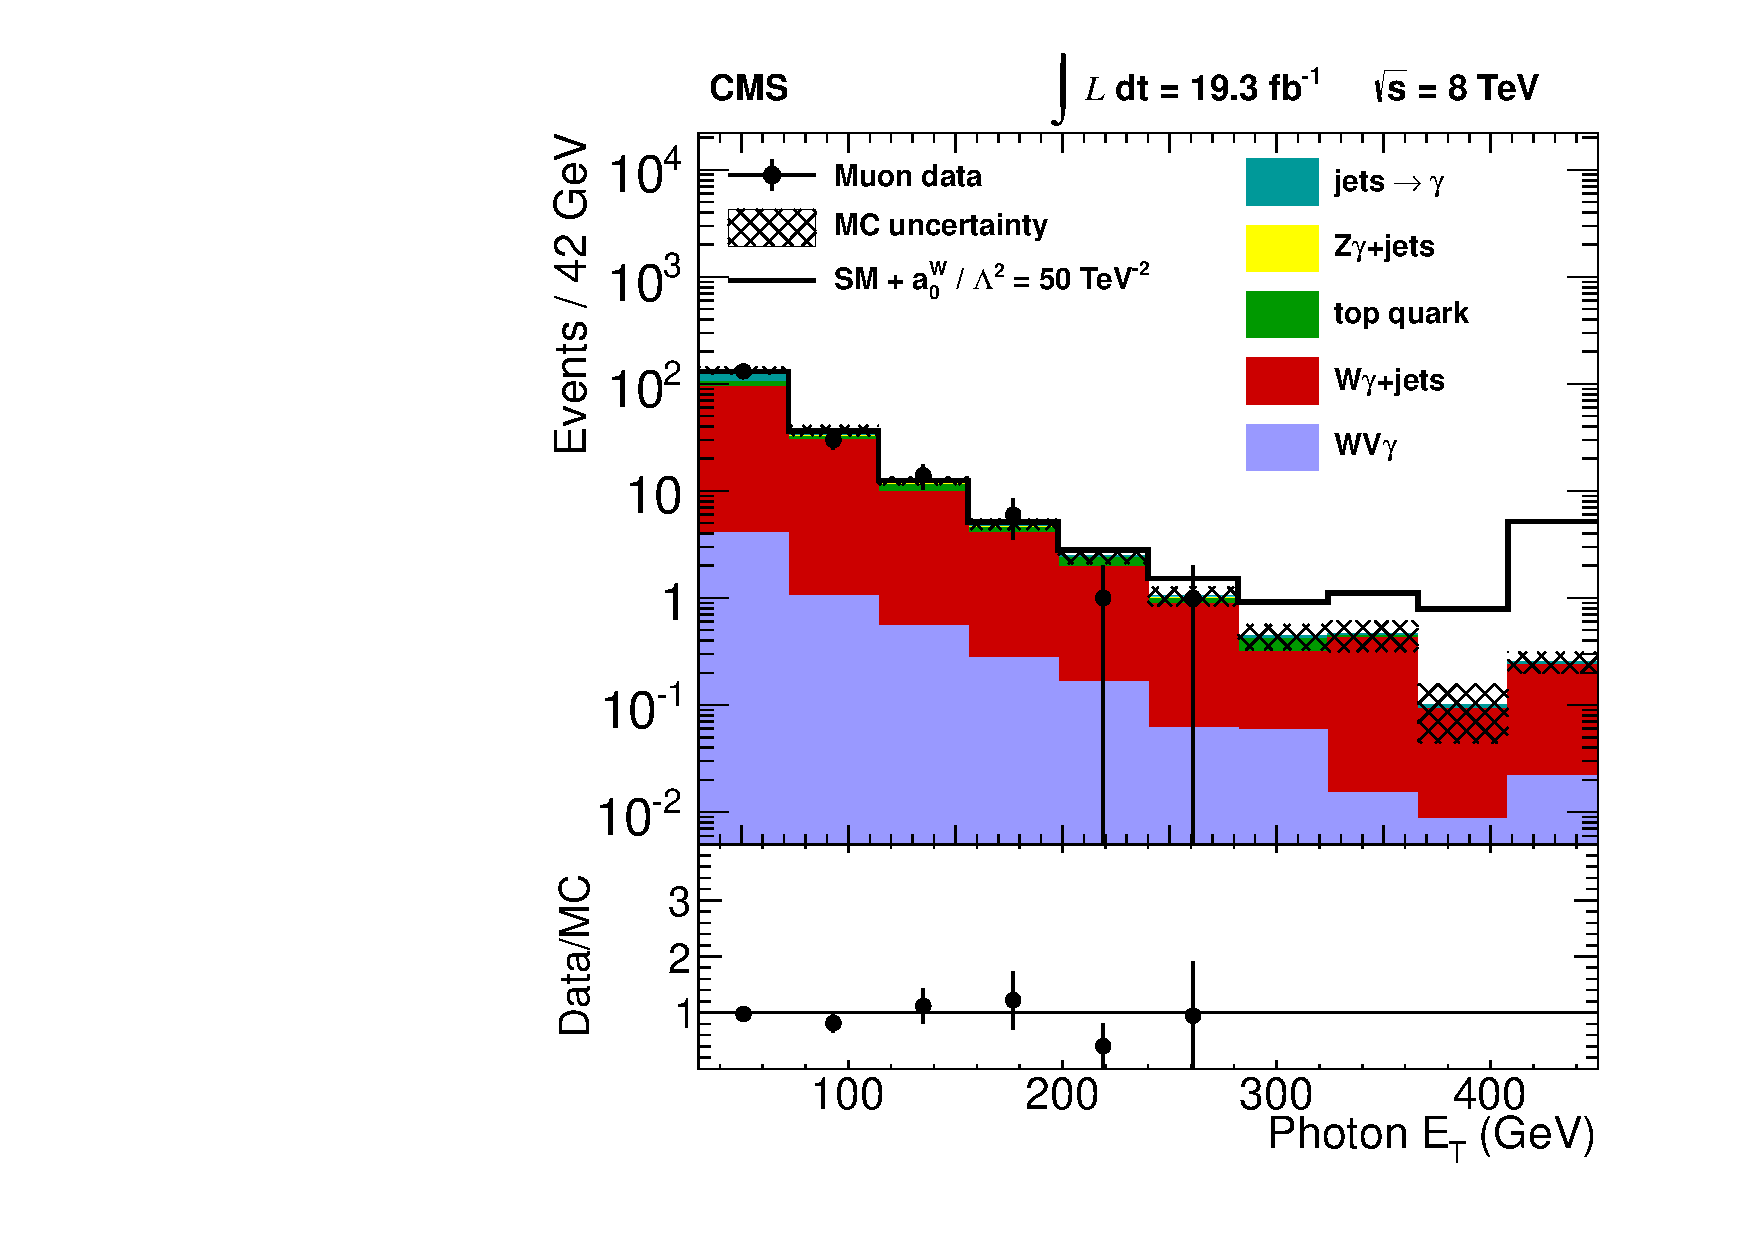
\includegraphics[width=0.45\textwidth]{figures/ss-inclboson-triboson-wvg-mu-cms8tev.pdf}
    \caption{}
    \label{fig:ss-inclboson-triboson-wvg-cms8tev}
\end{figure}


\section{Exclusive boson production}
\subsection{Exclusive single boson production, vector-boson fusion}
\begin{figure}[p]
    \centering
    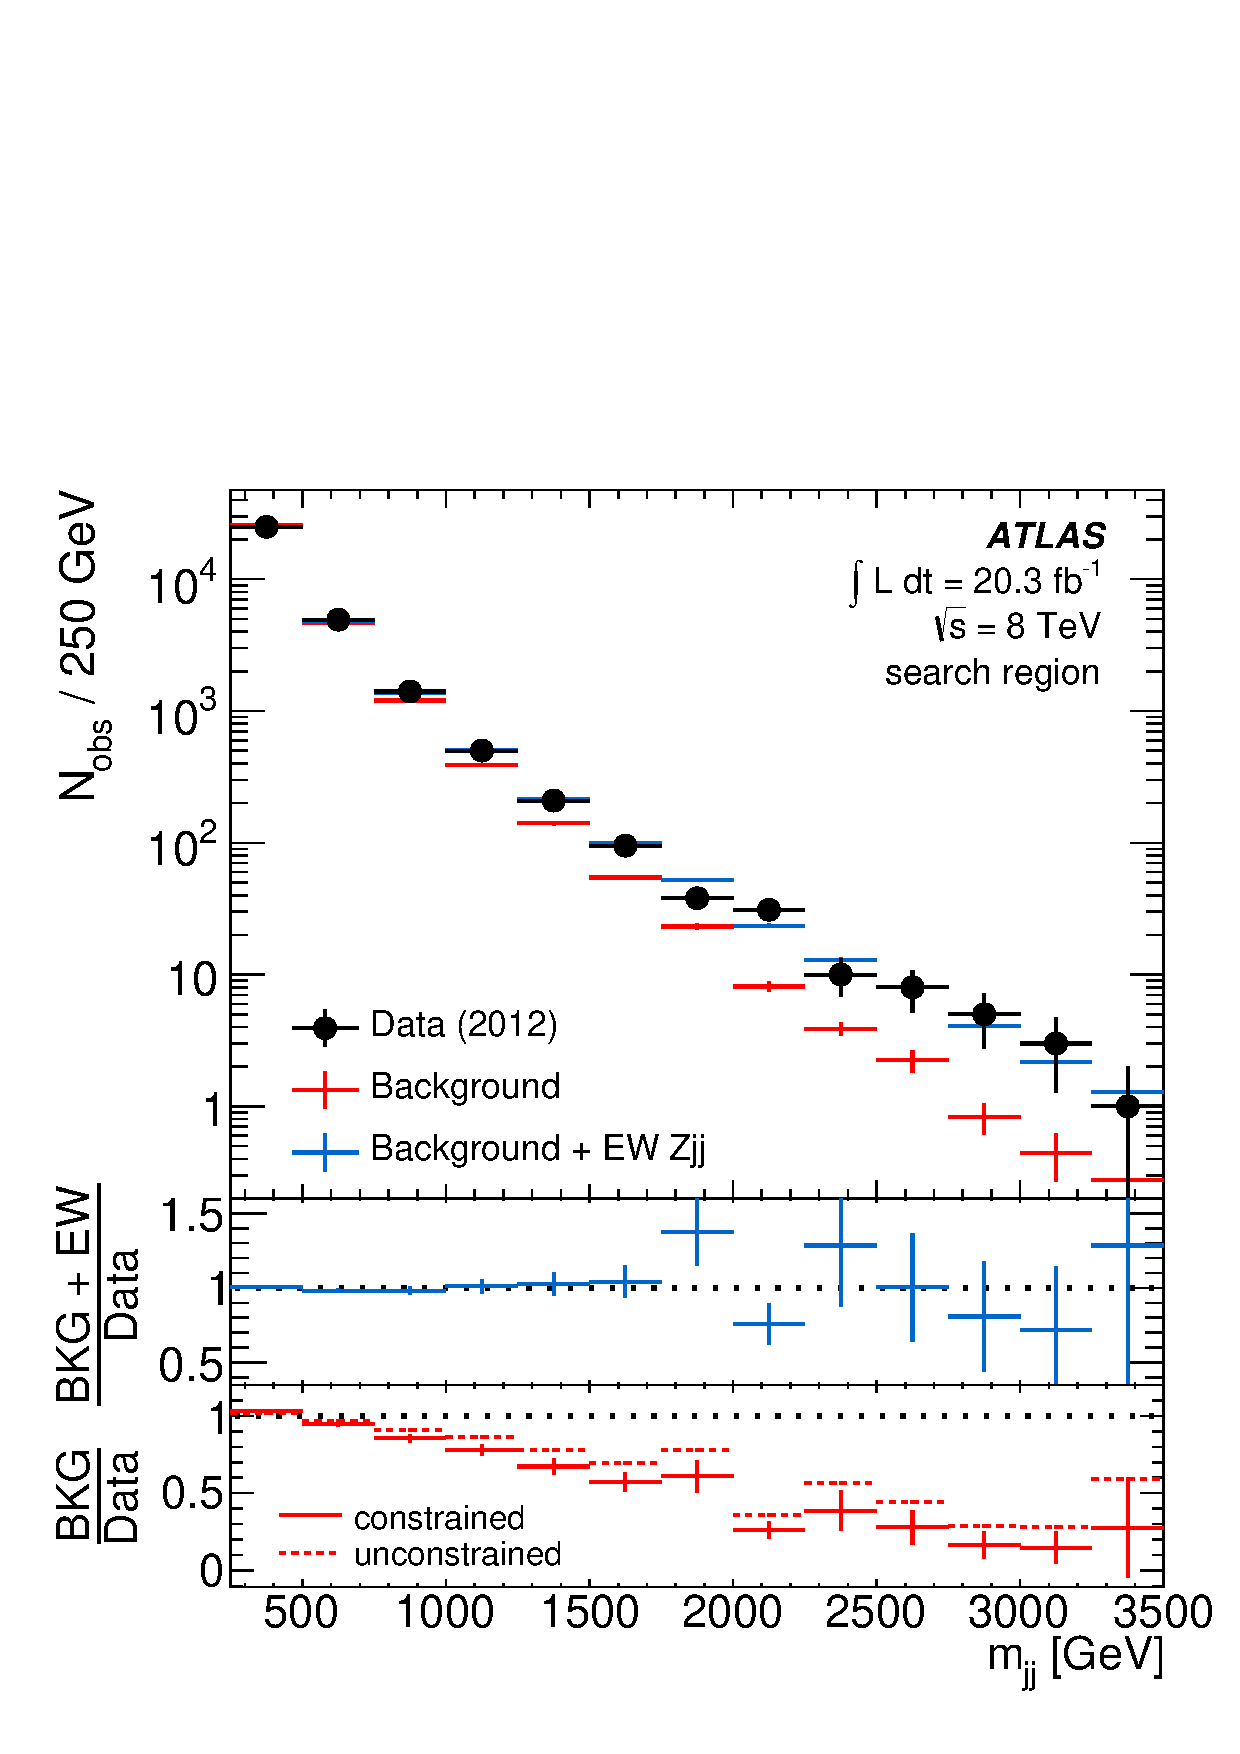
\includegraphics[height=0.3\textheight]{figures/ss-exclboson-z2j-atlas8tev}
    \caption{}
    \label{fig:ss-exclboson-z2j-atlas8tev}
\end{figure}
ATLAS VBF Z 7 \TeV~\cite{Aad:2014dta}

CMS VBF Z 7 \TeV~\cite{Chatrchyan:2013jya}

CMS VBF Z 8 \TeV~\cite{Khachatryan:2014dea}


\subsection{Exclusive di-boson production, vector-boson scattering}
%\begin{figure}[p]
%    \centering
%    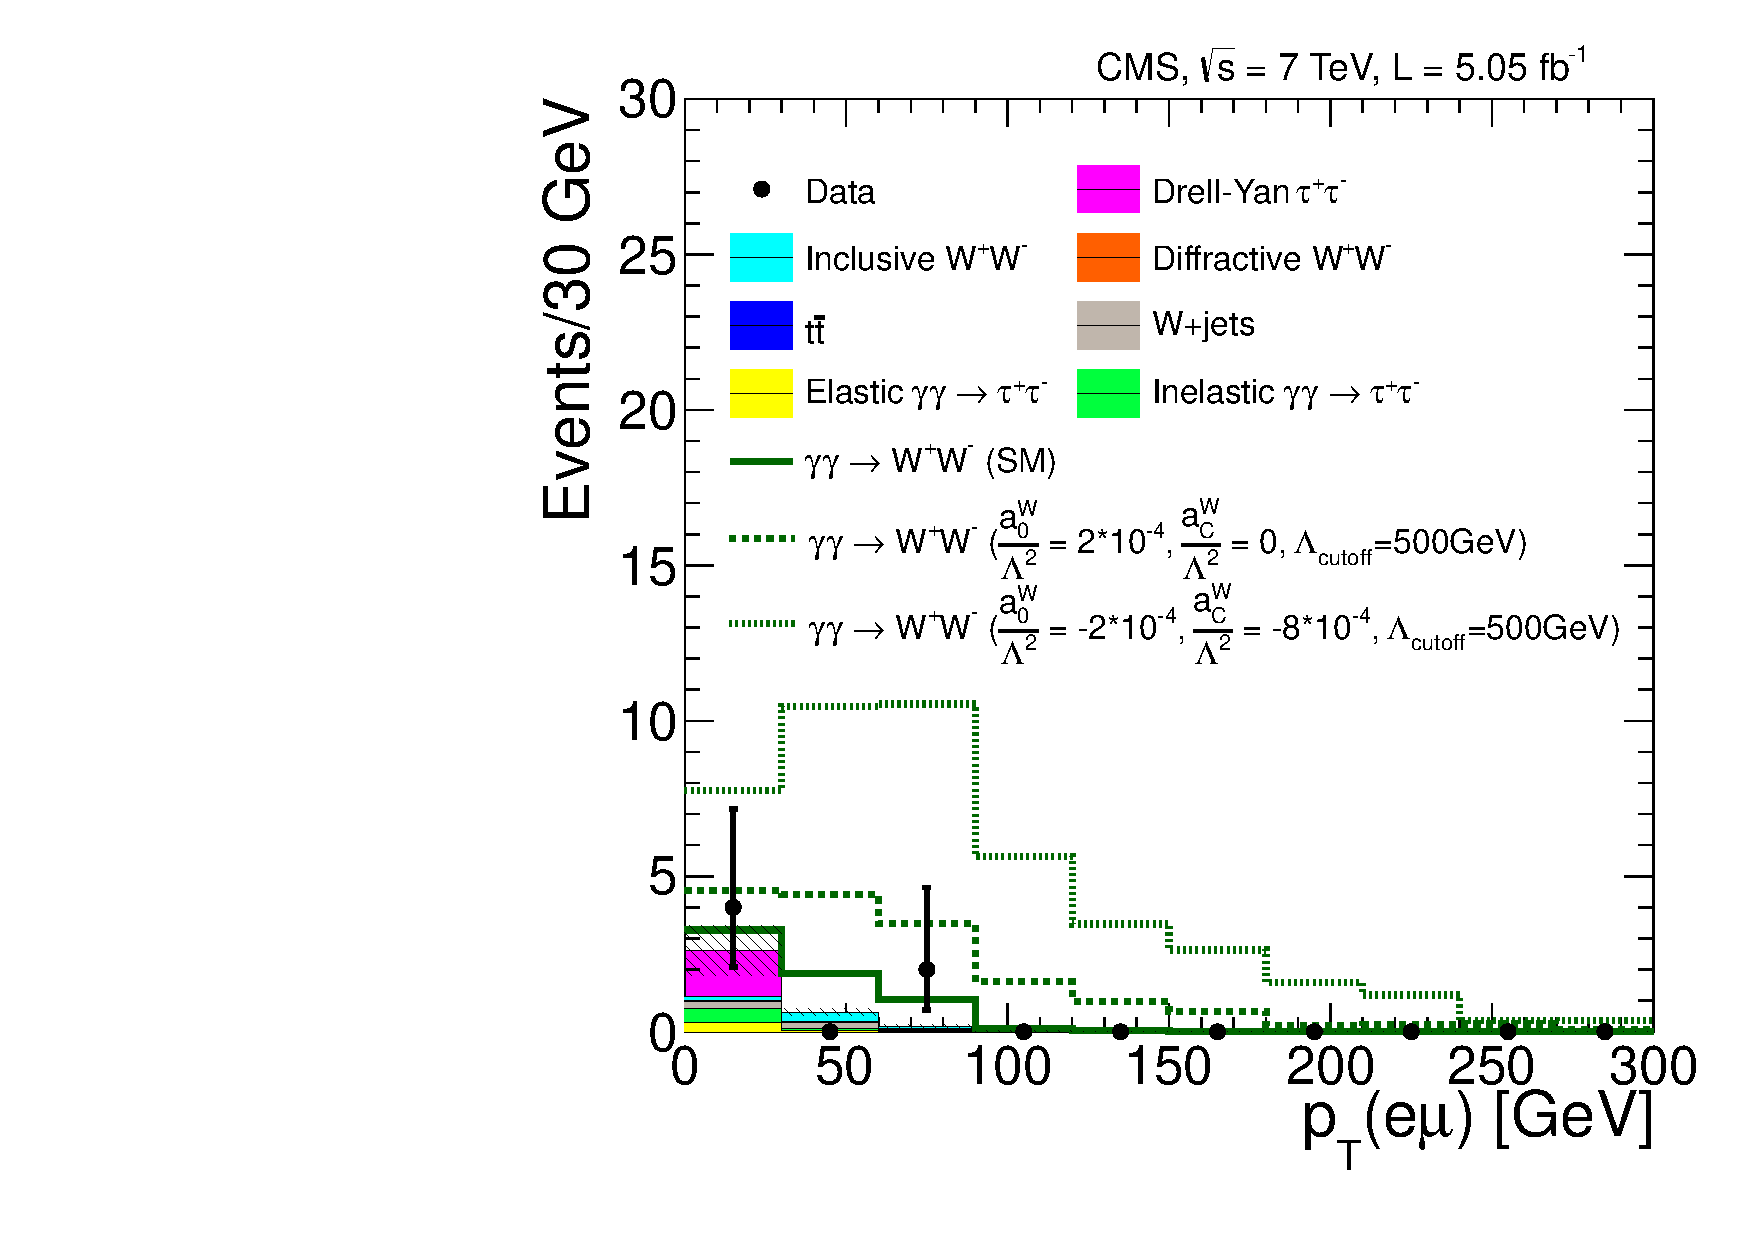
\includegraphics[height=0.3\textheight]{figures/ss-exclboson-ww-cms7tev}
%    \caption{}
%    \label{fig:ss-exclboson-ww-cms7tev}
%\end{figure}
%CMS WWexcl 7 \TeV~\cite{Chatrchyan:2013foa}

In addition to exclusive single boson production, CMS and ATLAS have
evidence for exclusive diboson production, in two different channels.
In one of them, CMS~\cite{Khachatryan:2016mud} has performed a search
for exclusive diboson production via protons emitting (possibly
quasi-) real photons which rescatter to produce $W^+W^-$ pairs:
$pp \to p^{(*)}W^+ W^- p^{(*)} \to p^{(*)}\mu^{\pm}e^{\mp}p^{(*)}$,
where $p^*$ admits the possibility that the protons dissociate into an
undetected system.  Such production is characterized by a
$\mu^{\pm}e^{\mp}$ pair which has no underlying event activity typical
of proton-proton hard scattering.  By selecting a $\mu^{\pm}e^{\mp}$
pair of sufficiently high individual (20 GeV) and joint (30 GeV)
transverse momentum, and requiring further that the two lepton tracks
intersect with each other, but have no additional tracks nearby, an
exclusive production signal is isolated from backgrounds such as
exclusive Drell-Yan and inclusive dilepton production from various
hard scattering mechanisms, respectively.  Selection efficiency is
validated by examining a control sample of exclusive same-flavor
Drell-Yan production ($p^{(*)}\mu^{\pm}\mu^{\mp}p^{(*)}$ or
$p^{(*)}e^{\pm}e^{\mp}p^{(*)}$) and comparing it with simulated
efficiency.  The relative contribution of dissociated proton
scattering for signal is also deduced by comparing the observed
exclusive Drell-Yan cross section with an exclusive matrix element
calculation (\texttt{LPAIR}~\cite{Vermaseren:1982cz,Baranov:1991yq});
proton dissociation is estimated to enhance the signal by a factor of
$4.10 \pm 0.43$ with respect to an exclusive calculation
from \texttt{MadGraph}.

Figure~\ref{fig:ss-exclboson-ww-cms8tev} shows the distributions of
dilepton $\pt$ and extra tracks in data compared with expectations
from simulation.  13 events are observed with an expected background
of $3.9\pm0.6$ in the 8 TeV data.  In the 7
TeV~\cite{Chatrchyan:2013foa} and 8 TeV data combined, a 3.4 $\sigma$
excess is observed over background as evidence for exclusive (plus
dissociative) $W^+W^-$ production.  The signal corresponds to a cross
section in the 8 TeV data of $11.9^{+5.6}_{-4.5}$ fb, in agreement
with a SM prediction of $6.9\pm0.6$ fb.  Exclusive $W^+W^-$ production
is sensitive to $WW\gamma\gamma$ quartic couplings. The CMS analysis
derived limits on the dimension 6 couplings $a^W_0/\Lambda^2$ and
$a^W_C/\Lambda^2$ and, in the context of dimension 8 EFT, the
anomalous couplings $f_{M(0,1,2,3)}/\Lambda^4$.  The 95\% CL upper
limits are $1.1(4.4)\times 10^{-4} \rm{GeV}^{-2}$ for
$a^W_0/\Lambda^2$ ($a^W_C/\Lambda^2$), and range from $2-17 \times
10^{-4} \rm{GeV}^{-4}$ for dimension 8 couplings, for models with no
form factor.  This process is the single best constraint on
$WW\gamma\gamma$ QGCs.

\begin{figure}[htb]
\centering
%\includegraphics[width=.48\textwidth]{Figures/2016_01_29_UpdatedPlots/ee_pt.pdf}
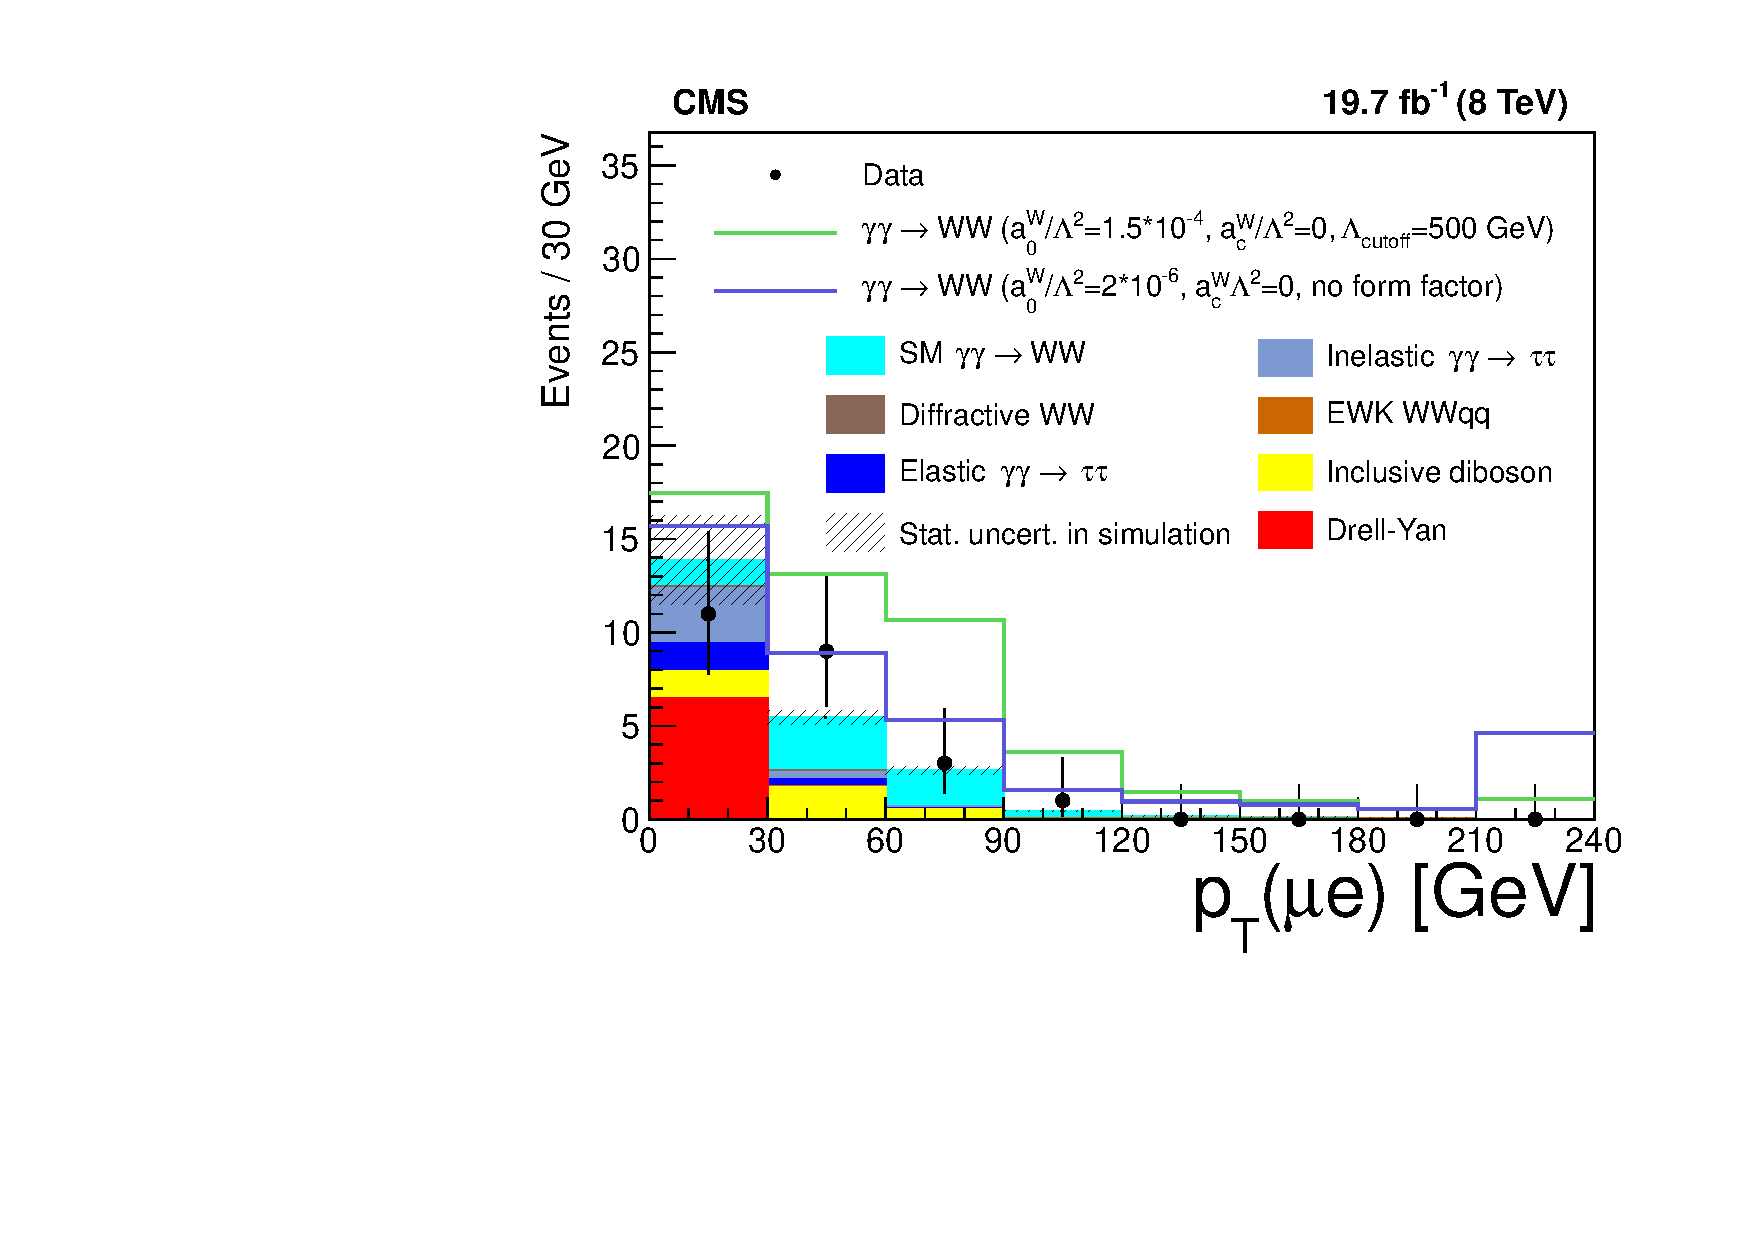
\includegraphics[width=.48\textwidth]{figures/ss-exclboson-ww-cms8tev-1.pdf}
%\includegraphics[width=.48\textwidth]{Figures/2016_01_29_UpdatedPlots/ee_tracks_
%pt30.pdf}
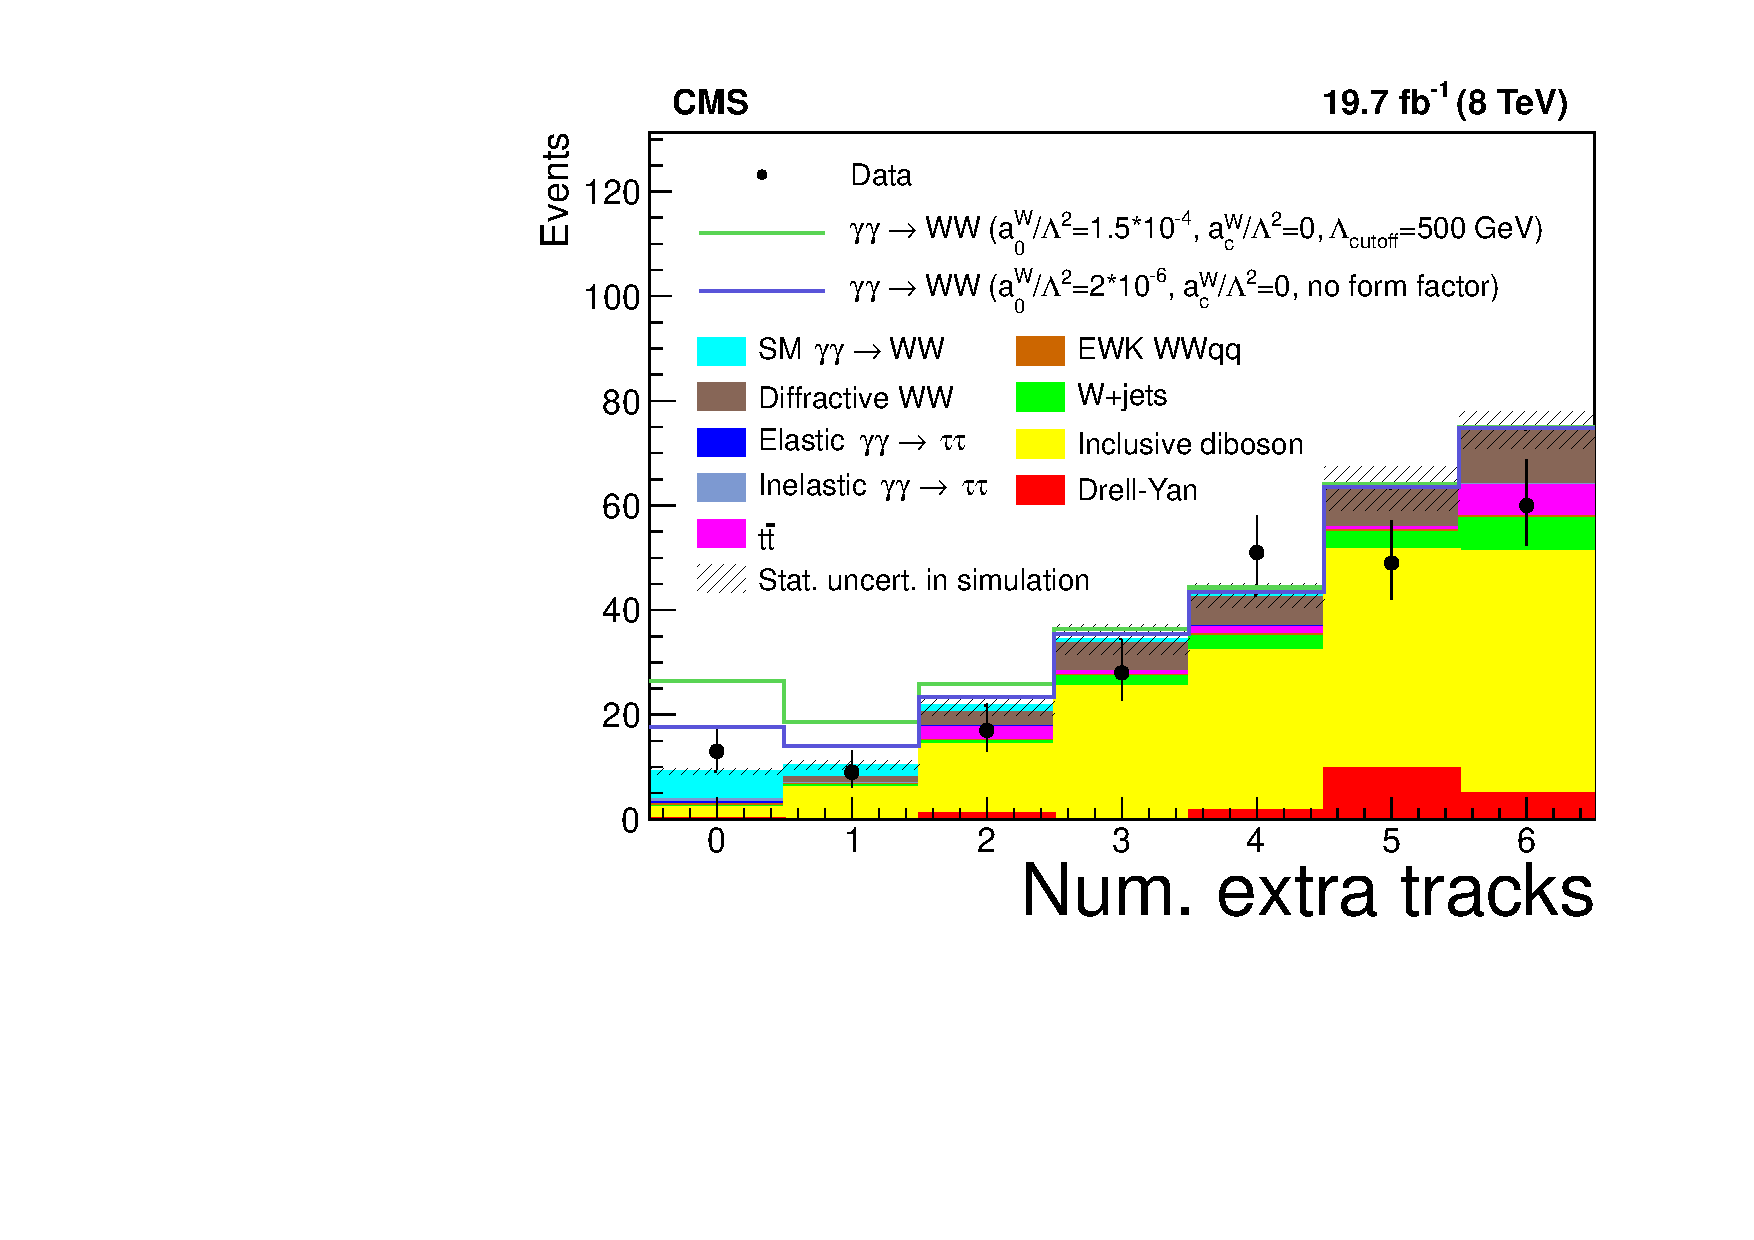
\includegraphics[width=.48\textwidth]{figures/ss-exclboson-ww-cms8tev-2.pdf}
\caption{Evidence for exclusive diboson production via $pp \to p^{(*)}W^+ W^- p^{(*)} \to p^{(*)}\mu^{\pm}e^{\mp}p^{(*)}$~\cite{Khachatryan:2016mud}.
Distributions of muon-electron transverse momentum for events with zero
 associated tracks (left), and extra-tracks multiplicity for events with $\pt(\mu^{\pm}e^{\mp}) > 30$ GeV (right).
 The data are shown by the points with error bars; the histograms indicate the expected SM signal and backgrounds.
\label{fig:ss-exclboson-ww-cms8tev}}
\end{figure}

The other exclusive diboson process for which the LHC has evidence is
same-sign $WW$ production, via the process $qq \to WW +
2q \to \ell^\pm\ell^\pm + 2 \rm{jet} + \met$.  Similar to exclusive
single boson production, the final state of interest is a
superposition of several amplitudes at leading order, some of which
are purely electroweak and include triple and quartic gauge boson
interactions (see Fig.~\ref{fig:ss-exclboson-ww-sigdiagram}), and
some of which have the final state jets arise from QCD initial- and
final-state radiation. Through a suitable choice of final state phase
space, the electroweak amplitudes are enhanced and the associated
signal strength and distributions can be tested against the
electroweak theory.  The same-sign $WW$ final state has the advantage
over other exclusive diboson channels ($\WW$ or $\WZ$) of a smaller
relative QCD amplitude and smaller multi-lepton backgrounds from top
quark, Drell-Yan, and $\WZ$ processes due to the same-sign dilepton
requirement.

An ATLAS analysis~\cite{Aad:2014zda} selects an ``inclusive region''
which is an admixture of electroweak and QCD contributions, and a VBS
signal region which is predominantly electroweak.  The inclusive
region requires two same-sign leptons with $\pt > 25$ GeV, $\met > 40$
GeV, and at least two jets with $m_{jj} > 500$ GeV for the two highest
$\pt$ jets; the VBS region further requires that the two highest $\pt$
jets are separated in rapidity, $|\Delta y_{jj}| > 2.4$.  To reduce
Drell-Yan background, events with dilepton mass less than 20 GeV or
dielectrons within 10 GeV of the $\Zzero$ mass are vetoed.  Top quark
background is reduced by vetoing events with b-tagged jets. Finally,
$WZ$ background is reduced by vetoing events with a third lepton with
muon $\pt > 6$ GeV or electron $\pt > 7$ GeV.  This results in 50
events selected for the inclusive region (as shown in
Fig.~\ref{fig:ss-exclboson-ww-ss}) and 34 for the VBS region.  About
half of selected events in either region are backgrounds from $\WZ$,
$W\gamma$ with photon conversion, and misidentified leptons from jets
in $V$ + jet processes.  The significance of the signal in the
inclusive region is observed (expected) to be 4.5$\sigma$
(3.4$\sigma$), and for the VBS region the significance is observed
(expected) to be 3.6$\sigma$ (2.8$\sigma$).  The measured cross
sections in these two regions are $2.1\pm 0.5\rm{(stat)} \pm
0.3\rm{(syst)}$ fb and $1.3 \pm 0.4\rm{(stat)}\pm 0.2\rm{(syst)}$ fb,
comparing well with SM predictions
from \texttt{Powheg-Box}~\cite{Nason:2004rx,Frixione:2007vw,Alioli:2010xd,Jager:2009xx,Melia:2010bm,Melia:2011gk}
of $1.52 \pm 0.11$ fb and $0.95\pm 0.06$ fb, respectively.

The VBS cross section is used to constrain parameters of an effective
chiral Lagrangian theory of vector boson
scattering~\cite{Alboteanu:2008my}, calculated
by \texttt{Whizard}~\cite{Kilian:2007gr,Moretti:2001zz}: $−0.14
< \alpha_4 < 0.16$ and $−0.23 < \alpha_5 < 0.24$ limits are obtained
at 95\% CL.

A CMS analysis~\cite{Khachatryan:2014sta} selects events similar to
the ATLAS VBS region: two same-sign leptons with $\pt>20$ GeV, two
jets with $m_{jj}>500$ GeV and $|\Delta \eta_{jj}| > 2.5$, and $\met >
40$ GeV.  There is a same-flavor Drell-Yan veto for events with
dilepton mass less than 50 GeV or dielectrons within 15 GeV of the Z
mass, a veto of top-like events with secondary vertex or soft muon
tags, and a third lepton veto for $\pt > 10$ GeV.  The 12 events so
selected are shown in Fig.~\ref{fig:ss-exclboson-ww-ss}.  About half
of them are expected to be background, mostly from misidentified
leptons. The resulting excess has a significance of 1.9$\sigma$
(2.9$\sigma$) observed (expected) for the purely electroweak
amplitude.  The observed fiducial cross section is
$4.0^{+2.4}_{−2.0} \rm{(stat)} ^{+1.1}_{−1.0} \rm{(syst)}$ fb compared
to an expected cross section estimated from \texttt{VBFNLO}~\cite{Baglio:2014uba,Arnold:2011wj,Arnold:2008rz} of
$5.8 \pm 1.2$ fb.

The $m_{\ell\ell}$ distribution of selected events is used to obtain
95\% CL bounds on dimension 8 EFT couplings $f_{S,(0,1)}$,
$f_{M,(0,1,6,7)}$, and $f_{T,(0,1,2)}$~\cite{Eboli:2006wa}.  For
$f_{S,(0,1)}$, which can correspond to a spin-one VBS resonance, the
limits are $-42 \rm{TeV}^{-4} < f_{S,0}/\Lambda^4 < 43 \rm{TeV}^{-4}$
and $-129 \rm{TeV}^{-4} < f_{S,1}/\Lambda^4 < 131 \rm{TeV}^{-4}$.

\begin{figure*}[htb] {
\centering
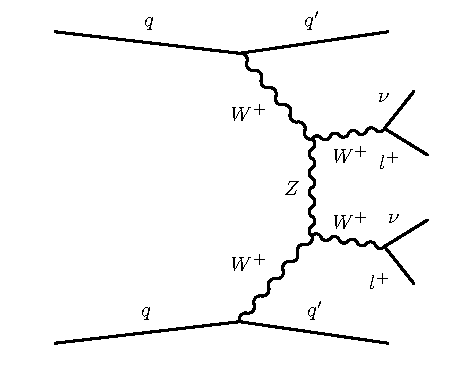
\includegraphics[width=0.315\textwidth]{figures/ss-exclboson-ww-diagram1.pdf}
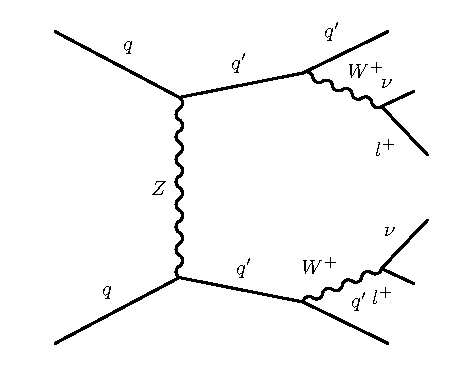
\includegraphics[width=0.35\textwidth]{figures/ss-exclboson-ww-diagram2.pdf}
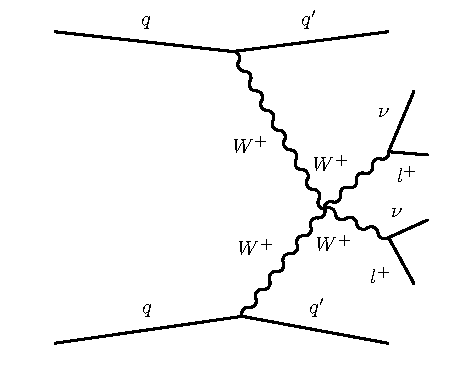
\includegraphics[width=0.315\textwidth]{figures/ss-exclboson-ww-diagram3.pdf}
\caption{
Representative Feynman diagrams for same-sign $WW$ production in association
with two jets from purely electroweak contributions:
(left) vector boson fusion,
(middle) bremsstrahlung-like,
and (right) multiperipheral production~\cite{Khachatryan:2014sta}.
\label{fig:ss-exclboson-ww-sigdiagram}}

}
\end{figure*}


\begin{figure}[p]
    \centering
    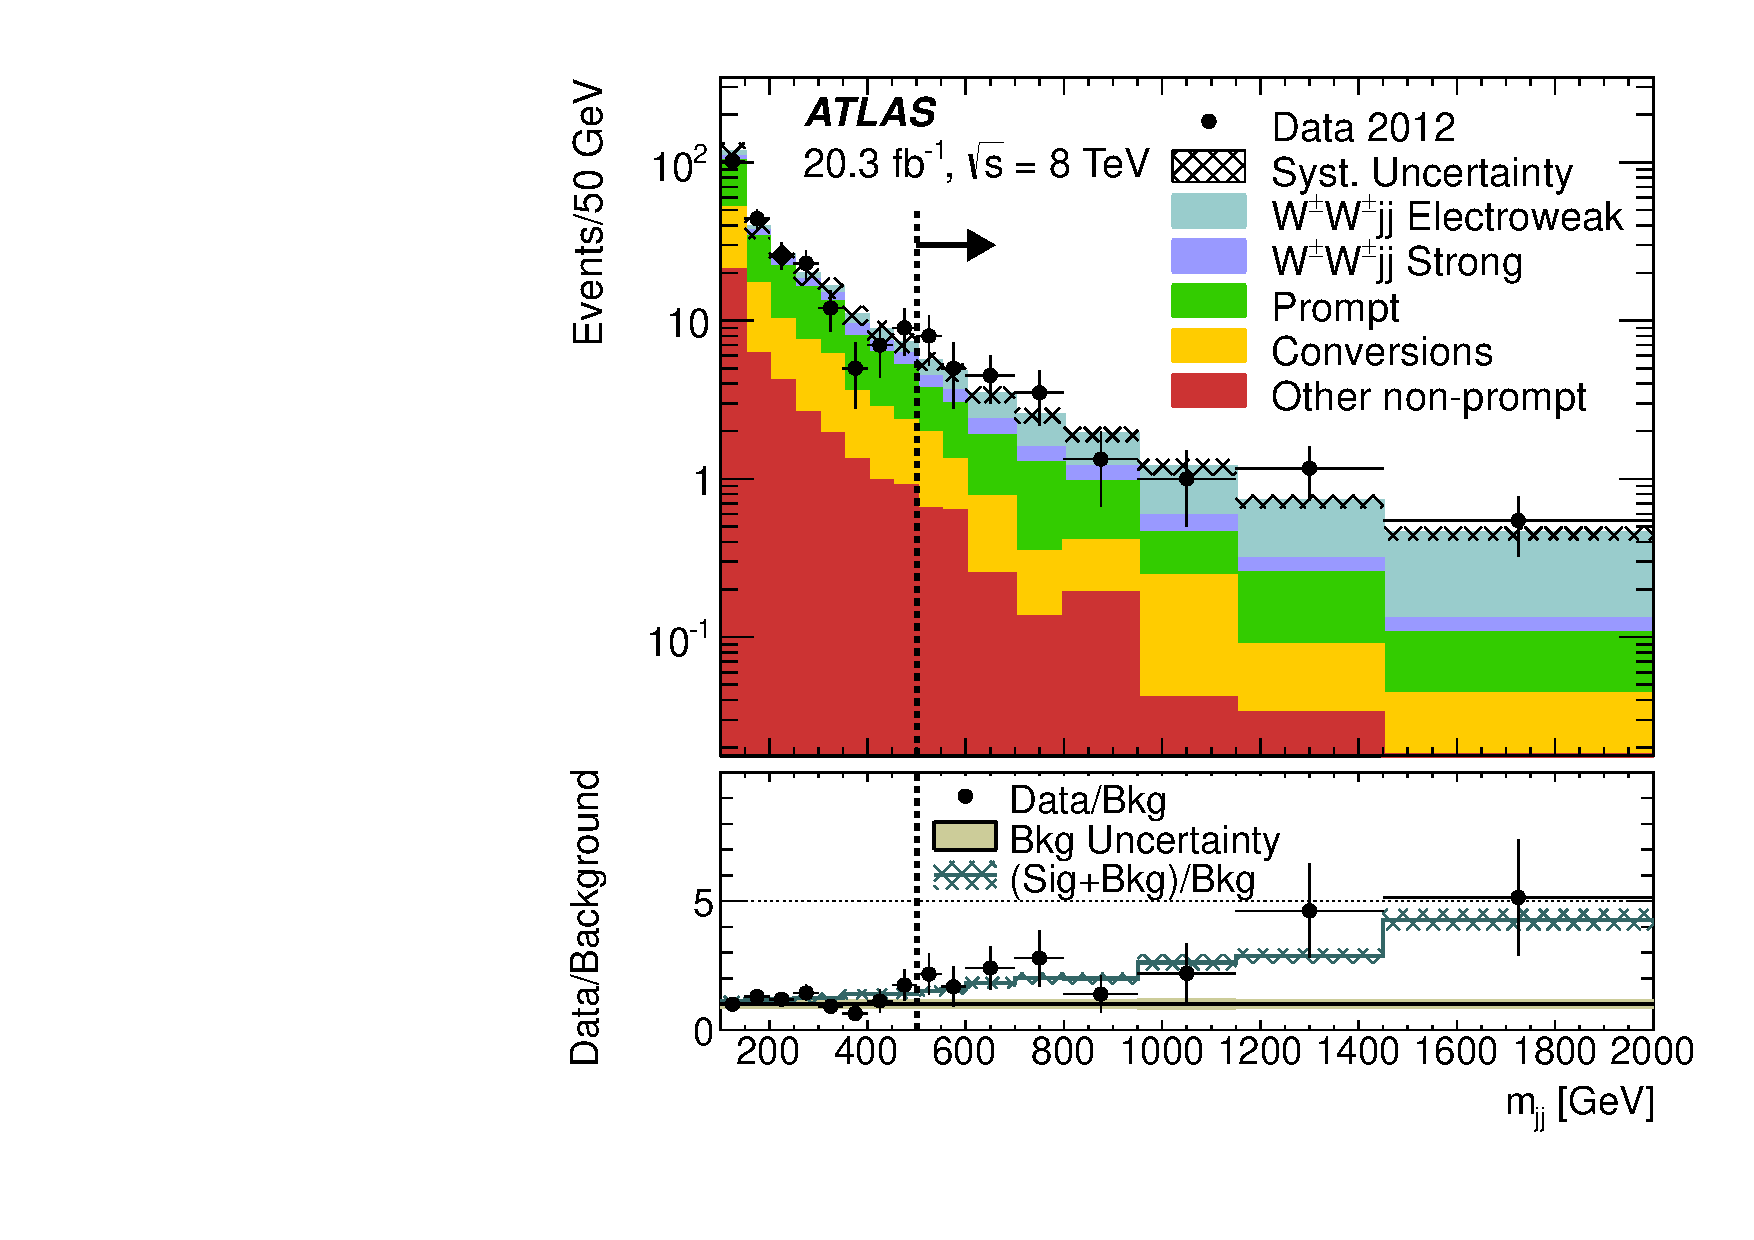
\includegraphics[width=0.45\textwidth]{figures/ss-exclboson-ww-ss-atlas8tev.pdf}
    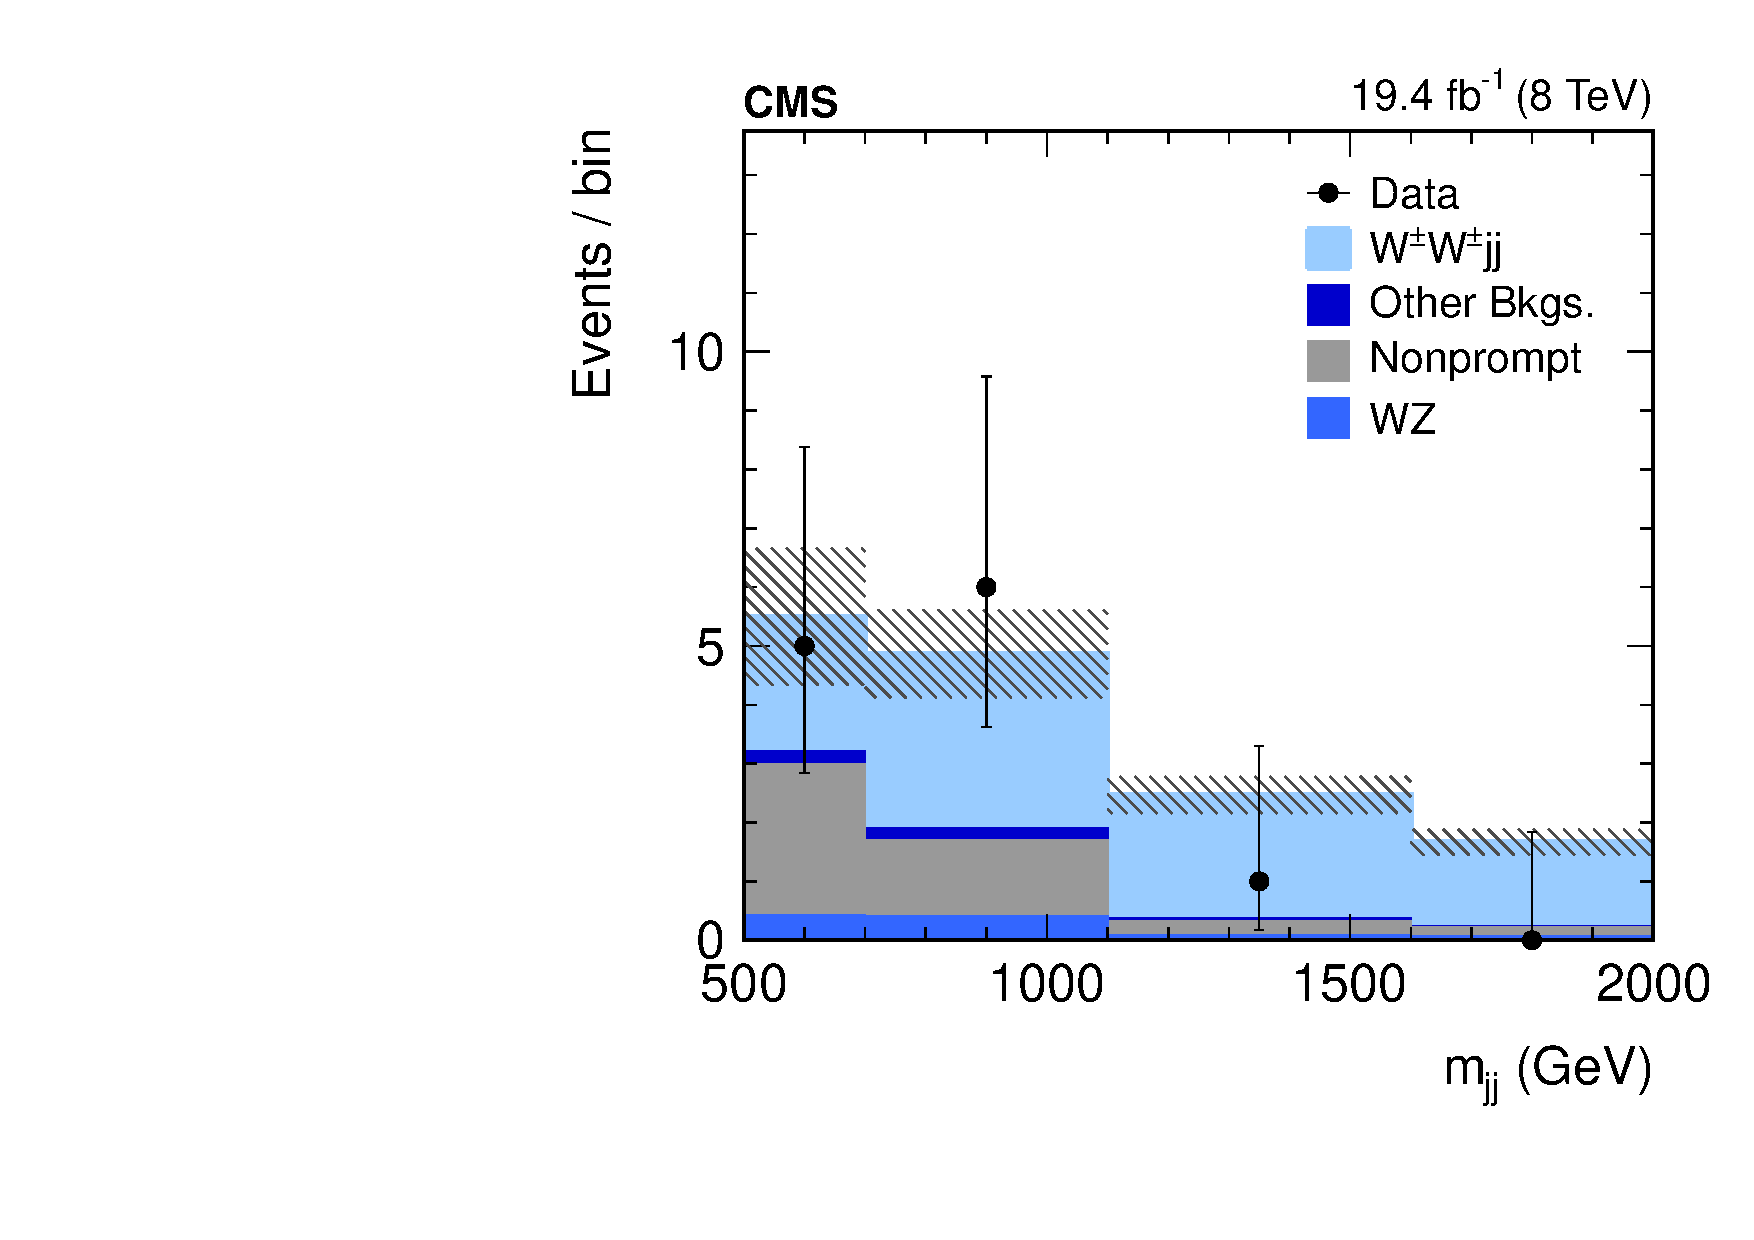
\includegraphics[width=0.45\textwidth]{figures/ss-exclboson-ww-ss-cms8tev.pdf}
    \caption{
    Left: Dijet invariant mass distribution of $W^{\pm} W^{\pm} jj$ candidates selected by ATLAS~\cite{Aad:2014zda}.  The inclusive signal region is indicated by the arrow.
    Right: Dijet invariant mass distribution of $W^{\pm} W^{\pm} jj$ candidates selected by CMS~\cite{Khachatryan:2014sta}.  }
    \label{fig:ss-exclboson-ww-ss}
\end{figure}


\section{Electroweak (precision) tests of the standard model}
\subsection{Test of tri-boson vertex}

ATLAS Wgamma Zgamma 7 \TeV~\cite{Aad:2013izg}

ATLAS WW 7 \TeV~\cite{ATLAS:2012mec}

ATLAS WW+WZ cross section 7 \TeV~\cite{Aad:2014mda}

ATLAS WZ 7 \TeV~\cite{Aad:2012twa}

ATLAS ZZ4l,ZZ2l2v 7 \TeV~\cite{Aad:2012awa}

CMS ZZ4l 8 \TeV~\cite{Khachatryan:2014dia}

CMS ZZ4l 7 \TeV~\cite{Chatrchyan:2012sga}

CMS WW2l2n 7 \TeV~\cite{Chatrchyan:2013yaa}

CMS WWlnjj 7 \TeV~\cite{Chatrchyan:2012bd}

CMS WW2l2n 8 \TeV (CMS-PAS-SMP-14-016, to be published)

CMS \Wg/\Zg 7 \TeV~\cite{Chatrchyan:2013fya}

CMS Znngamma 7 \TeV~\cite{Chatrchyan:2013nda}

CMS \Zg 8 \TeV~\cite{Khachatryan:2015kea}

CMS \ZZllvv 7+8 \TeV~\cite{Khachatryan:2015pba}

\subsection{Test of tetra-boson vertex}
ATLAS $W\gamma\gamma$ 8 \TeV~\cite{Aad:2015uqa}

ATLAS SSWW 8 \TeV~\cite{Aad:2014zda}

CMS WVgamma 8 \TeV~\cite{Chatrchyan:2014bza}

CMS WWexcl 7 \TeV~\cite{Chatrchyan:2013foa}

CMS SSWW 8 \TeV~\cite{Khachatryan:2014sta}

\begin{figure}[p]
    \centering
    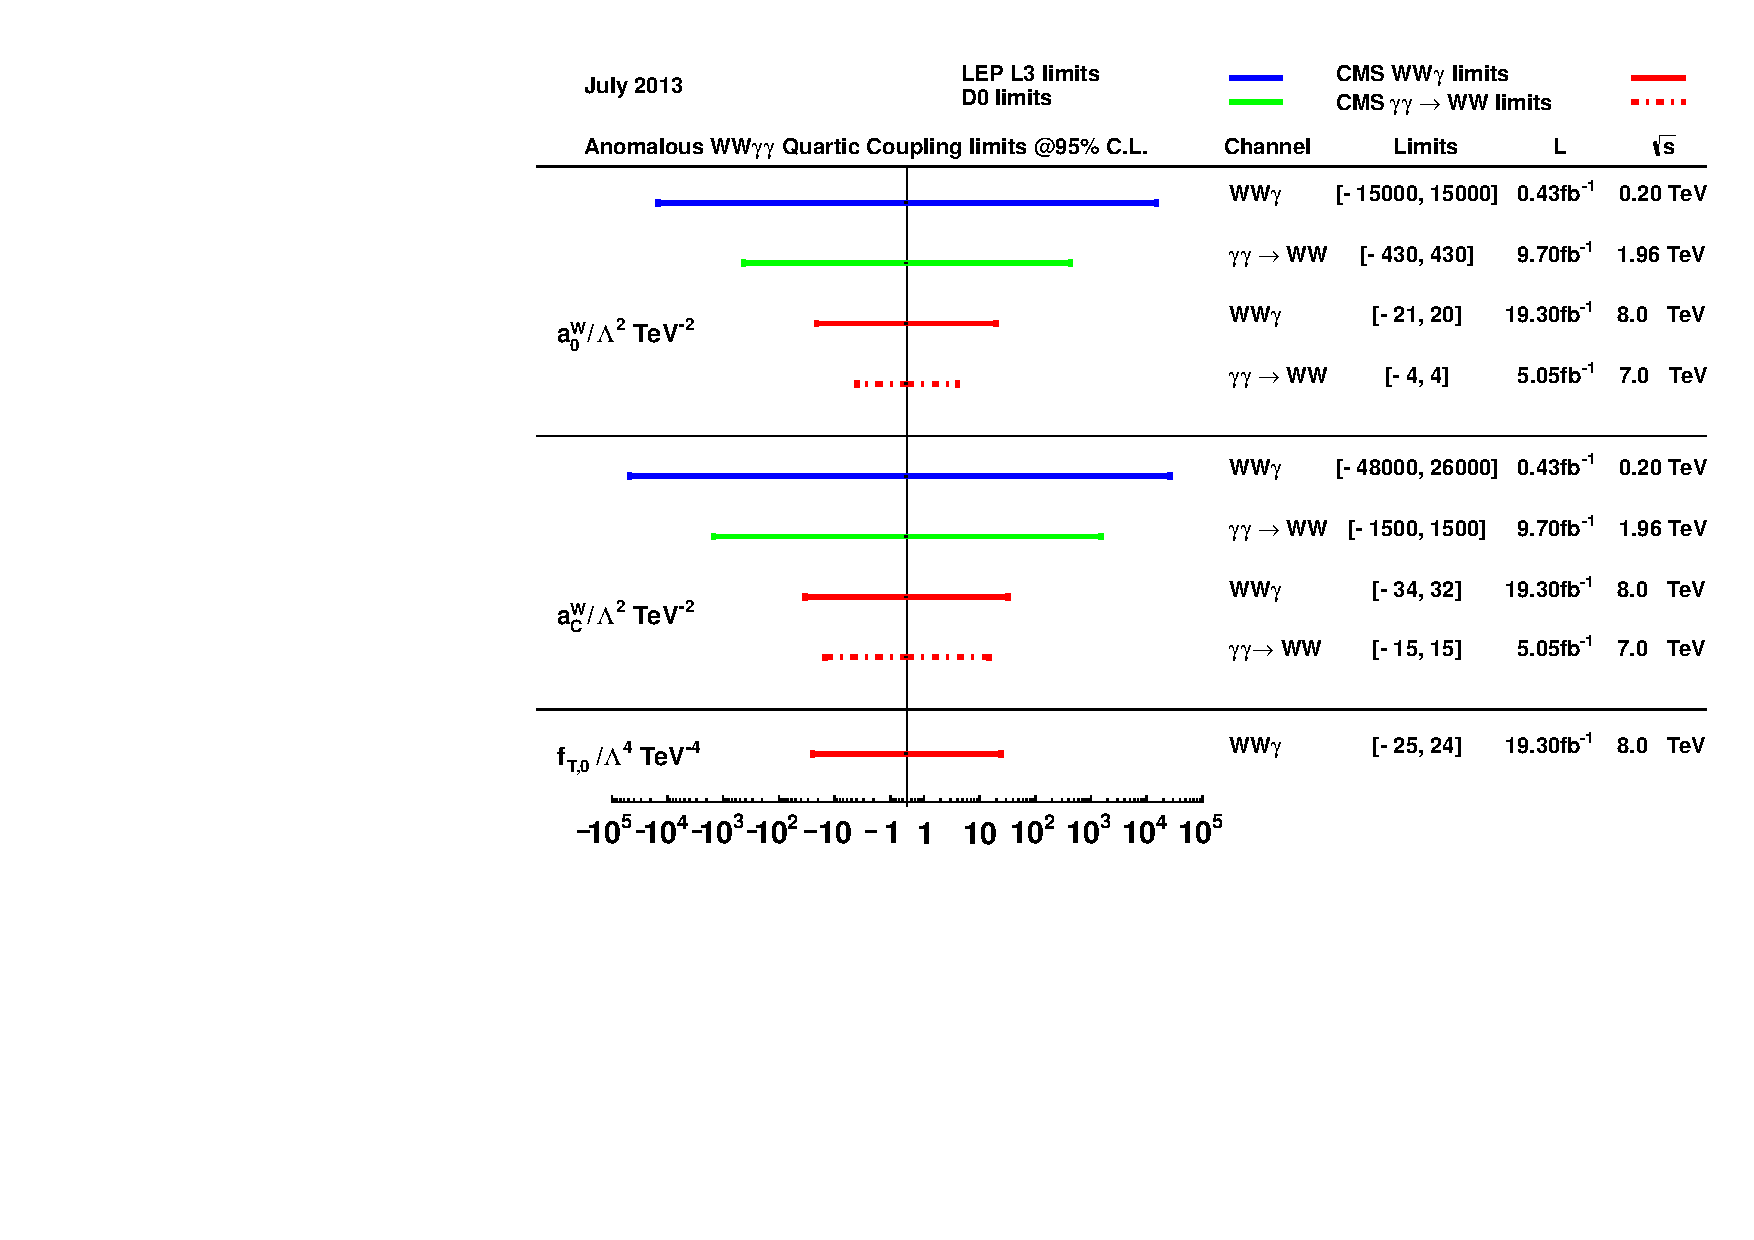
\includegraphics[height=0.3\textheight]{figures/ss-precision-qgc-wwgg.pdf}
    \caption{}
    \label{fig:ss-precision-qgc-wwgg}
\end{figure}


\subsection{Z AFB and sin thetaW}
%ATLAS weak mixing angle~\cite{Aad:2015uau}

In the electroweak theory the weak mixing angle $\theta_W$ is a free
parameter indicating the degree of mixing between $SU(2)_L$ and
$U(1)_Y$ neutral gauge bosons upon electroweak symmetry breaking to
obtain the physical neutral gauge bosons $\gamma$ and $\Zzero$.
Experimentally, it is typically measured as $\sin^2\theta_W$ via
angular distributions in fermion pair production; it has been most
precisely measured at the LEP 1 and SLD experiments via fermion pair
production at the $\Zzero$ pole, yielding a combined value of
$0.23153\pm0.00016$~\cite{ALEPH:2005ab}. In the standard model it is
related to the gauge boson masses at tree level by $1-m_W^2/m_Z^2$ and
modified by higher-order loop corrections, including contributions
from Higgs boson loops; the effective angle measured upon introducing
loop corrections is denoted as $\sin^2\theta^{eff}_{W}$. The recent
high-precision Higgs boson mass measurement at the LHC combined with
other electroweak measurements can be used to predict a value for
$\sin^2\theta^{eff}_{W}$ of $0.23149 \pm 0.00007$~\cite{Baak:2014ora},
motivating an improvement upon the direct experimental measurement
precision by a factor of two or more at the LHC to constrain the
electroweak theory further.

At a hadron collider, fermion pair production at and around the $\Zzero$
pole is measured in the process
$q\bar{q}\rightarrow \gamma^*/Z \rightarrow \ell^+\ell^-$, where the
differential scattering cross section is characterized by
$d^3\sigma/dm \ dy \ d\cos\theta = A(m,y)(1+\cos^2\theta) +
B(m,y)\cos\theta$, where $m$ is the final state lepton pair mass, $y$
is the lepton pair rapidity, and $\cos\theta$ is the polar angle of
the positive lepton with respect to the quark direction. A
non-vanishing forward-backward asymmetry in this angle, $A_{FB}(m,y) =
3B(m,y)/8A(m,y)$, arises from interference between vector and
axial-vector currents; the portion of $A_{FB}(m,y)$ corresponding to
self-interference of the $\Zzero$ boson currents is directly sensitive to
$\sin^2\theta^{eff}_{W}$.

In hadron collisions, the quark direction is ambiguous, as it may
originate from either incoming hadron and have unknown transverse
momentum. The impact of quark transverse momentum on the
forward-backward assignment is minimized by defining the quark
direction to be the difference between the forward-going and
backward-going hadron momentum vectors in the lepton pair rest frame,
as originally suggested by Collins and Soper~\cite{Collins:1977iv};
this angle is typically denoted as $\cos\theta^*$. In proton-proton
collisions, the ambiguity due to quark origination is an irreducible
dilution in $A_{FB}$ which is strongest at low $|y|$ and decreasing at
higher $|y|$ where valence quark/sea anti-quark annihilation is
predominant; measurements of $A_{FB}(m,y)$ at high-$|y|$ are therefore
intrinsically more sensitive to the undiluted value and have smaller
theory uncertainties related to PDFs.  In proton--anti-proton
collisions, valence quark/valence anti-quark annihilation
predominates, and so dilution and its associated uncertainties are
vastly reduced, making the Tevatron experimental
measurements~\cite{Aaltonen:2016nuy,Aaltonen:2014loa,Abazov:2014jti} a
competitive alternative to the LHC for current data samples. Three LHC
experiments have measured $\sin^2\theta^{eff}_{W}$: an initial
exploratory measurement by CMS at 7 TeV~\cite{Chatrchyan:2011ya}, a
measurement by ATLAS with all 7 TeV data~\cite{Aad:2015uau}, and a
measurement by LHCb~\cite{Alves:2008zz,Aaij:2014jba} with all 7 and 8
TeV data~\cite{Aaij:2015lka}.

The ATLAS measurement was performed with three different samples: muon
pairs with $\pt > 20$ GeV and $|\eta| < 2.4$; electron pairs with $E_T
> 25$ GeV and $|\eta| < 2.47$; and electron pairs with $E_T > 25$ GeV
where one has $|\eta| < 2.47$ and the other has $2.5 < |\eta| < 4.9$.
In the last case the forward electron is identified with calorimeters
alone, still the resulting pairs have a signal purity at the
$\Zzero$ pole of 95\%.  The data in each sample $i$ are binned in mass, and
the raw measured angular asymmetry in that region of phase space,
$A^{\rm meas}_{FB, i}(m)$, is computed from counting forward
($\cos\theta^* > 0$) and backward ($\cos\theta^* < 0$) candidates
after background subtraction.  Each $A_{FB,i}$ is used to extract
$\sin^2\theta^{eff}_{W}$ via a binned $\chi^2$ fit of
LO \texttt{PYTHIA} templates of different mixing angle values to the
data.  Figure~\ref{fig:ss-precision-afb-atlas-cf} shows the
$\cos\theta^*$ distribution for selected central-forward electron
pairs; an asymmetry between forward and backward angles is visually
evident.  Figure~\ref{fig:ss-precision-afb-atlas-cf} also show the
resulting $A^{\rm meas}_{FB}(m)$, alongside the best-fit predictions
from LO \texttt{PYTHIA} and NLO \texttt{POWHEG}.  The three samples
give consistent values for $\sin^2\theta^{eff}_{W}$ and are combined
to give a value of $0.2308 \pm 0.0005\textrm{(stat.)} \pm
0.0006\textrm{(syst.)} \pm 0.0009\textrm{(PDF)}$, where the last term
denotes the leading uncertainty in $\sin^2\theta^{eff}_{W}$ from
uncertainties in specially prepared LO PDFs consistent with the LO
PYTHIA template generation and 7 TeV ATLAS $W$ and $\Zzero$ data
(ATLAS-epWZ12 LO)~\cite{Aad:2011dm}.  A general feature of precision
electroweak measurements at the LHC is the predominance of PDF
uncertainties, requiring simultaneous PDF measurement with the
parameter of interest to obtain the best precision.  Other leading
systematic uncertainties are the lepton energy scale and MC template
statistics, which will improve with larger data sets.

The LHCb measurement employs a very similar technique.  They select
muon pairs with $\pt > 20$ GeV, $60 < m_{\mu\mu} < 160$ GeV, and $2.0
< |\eta| < 4.5$, with a signal mass resolution and purity similar to
ATLAS but in a more forward, and therefore more sensitive, $\Zzero$
production region.  LHCb operational instantaneous luminosity is
limited to the range $2-4\times
10^{32}\textrm{cm}^{-2}\textrm{s}^{-1}$, however, so the sample size
is limited to $1\;\fb^{-1}$ at 7~TeV and $2\;\fb^{-1}$ at 8 TeV.  The
data are binned in mass and $A_{FB}(m)$ is computed for their
acceptance, and then subsequently unfolded to account for mass
resolution effects. Figure~\ref{fig:ss-precision-afb-lhcb} shows the
unfolded $A_{FB}$ distribution at 8 TeV compared with NLO predictions
from \texttt{POWHEG-BOX}.  The unfolded $A_{FB}(m)$ distribution is
used to extract $\sin^2\theta^{eff}_{W}$ via a $\chi^2$ fit
of \texttt{POWHEG-BOX} templates of different mixing angle values to
the data.  They measure $\sin^2\theta^{eff}_{W} = 0.23142 \pm
0.00073 \textrm{(stat.)} \pm 0.00052 \textrm{(syst.)} \pm
0.00056 \textrm{(th.)}$, where the last term denotes uncertainties
from theoretical modelling ingredients, predominantly PDFs.  The PDF
uncertainties are evaluated from QCD+QED NLO NNPDF
2.3~\cite{Ball:2013hta,Ball:2012cx}, which, similar to the ATLAS PDF,
includes 7 TeV electroweak production data from the LHC.  In contrast
to the ATLAS result, the LHCb measurement statistically limited, but
has 30\% smaller theoretical uncertainties due to better understood
PDF uncertainties in the more forward production region.  In both
experiments, the impact of correctly modelling QED final state
radiation and higher-order electroweak corrections was studied via
comparison between different contemporary calculations, including
\texttt{PHOTOS}~\cite{Golonka:2005pn} and \texttt{PHOTONS++}~\cite{Schonherr:2008av} for
QED radiation, and \texttt{FEWZ}, \texttt{HORACE}~\cite{CarloniCalame:2007cd}, and
\texttt{POWHEG-BOX} for electroweak corrections.  The uncertainty associated
with these corrections is of order 0.1\% and sub-leading compared to
PDFs.

A comparison of experimental measurements of
$\sin^2\theta^{eff}_{W}$~\cite{Aaltonen:2016nuy} is shown in
Figure~\ref{fig:ss-precision-summary-sin2thetaw}.  The best single
measurements from the Tevatron are more than twice as precise as the
best measurements from the LHC, and the separate $A^{0,b}_{FB}$ and
$A_{l}$ results from $e^+e^-$ collisions are more than four times as
precise.  There are reasonable prospects for the LHC experiments
eventually surpassing these: ATLAS and CMS are expected to have
superior statistical uncertainties by the end of Run 2, and all of the
systematic and PDF uncertainties are expected to improve as well with
larger electroweak data samples.

%CMS Drell--Yan AFB 7 \TeV~\cite{Chatrchyan:2012dc}
%CMS Drell--Yan AFB 8 \TeV (CMS-PAS-SMP-14-004, to be published)
\begin{figure}[p]
    \centering
    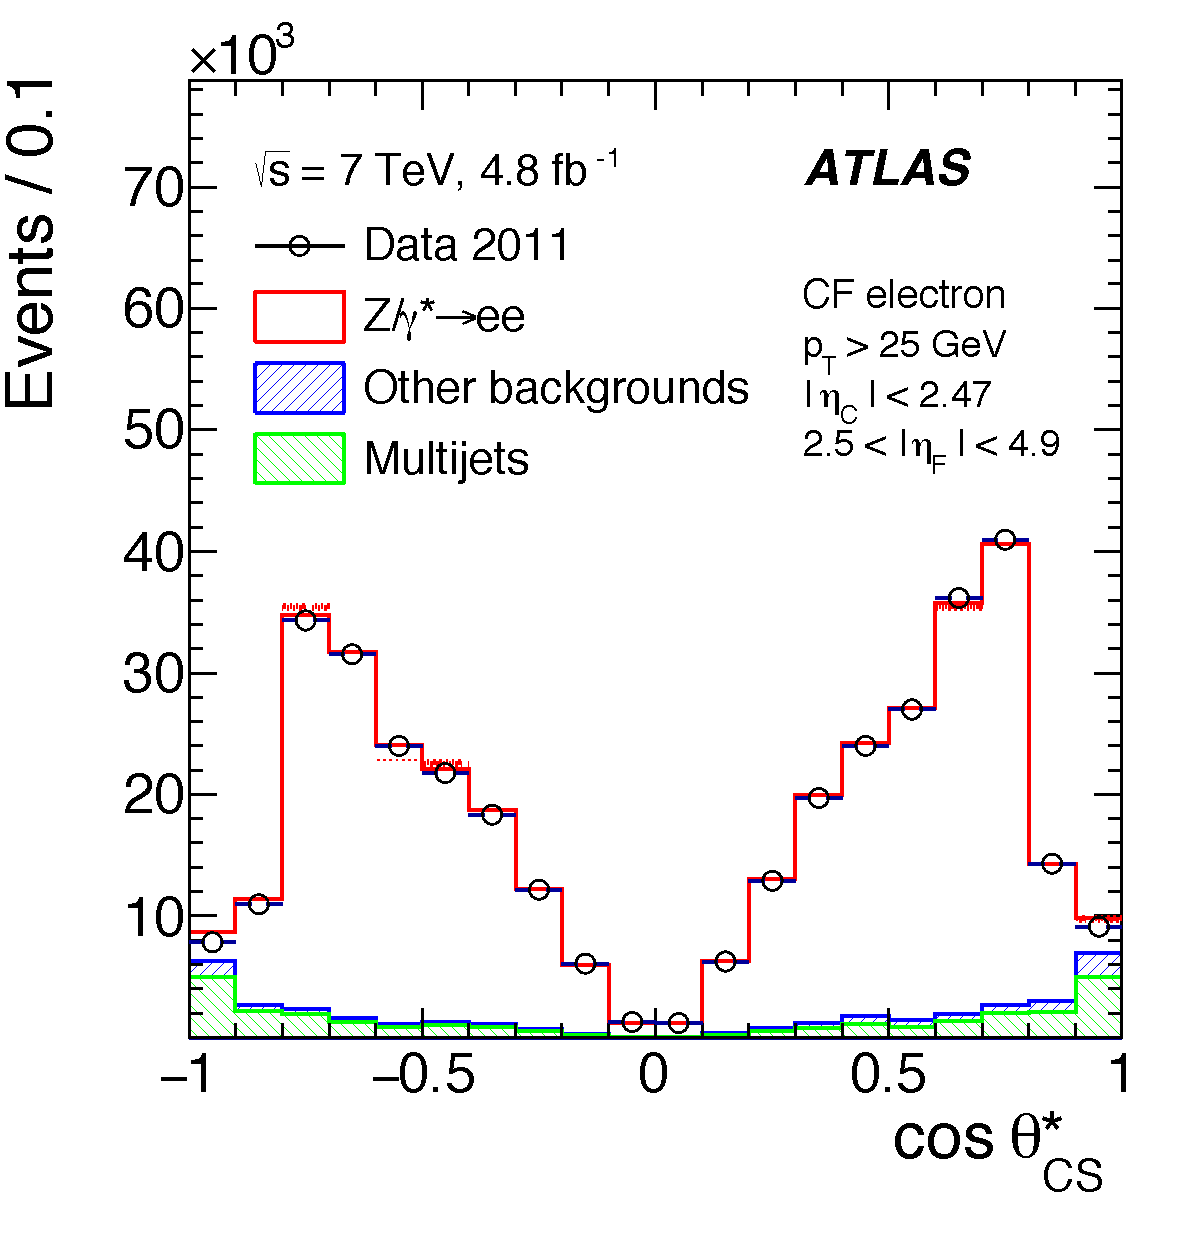
\includegraphics[width=0.45\textwidth]{figures/ss-precision-afb-atlas-cf-ct.pdf}
    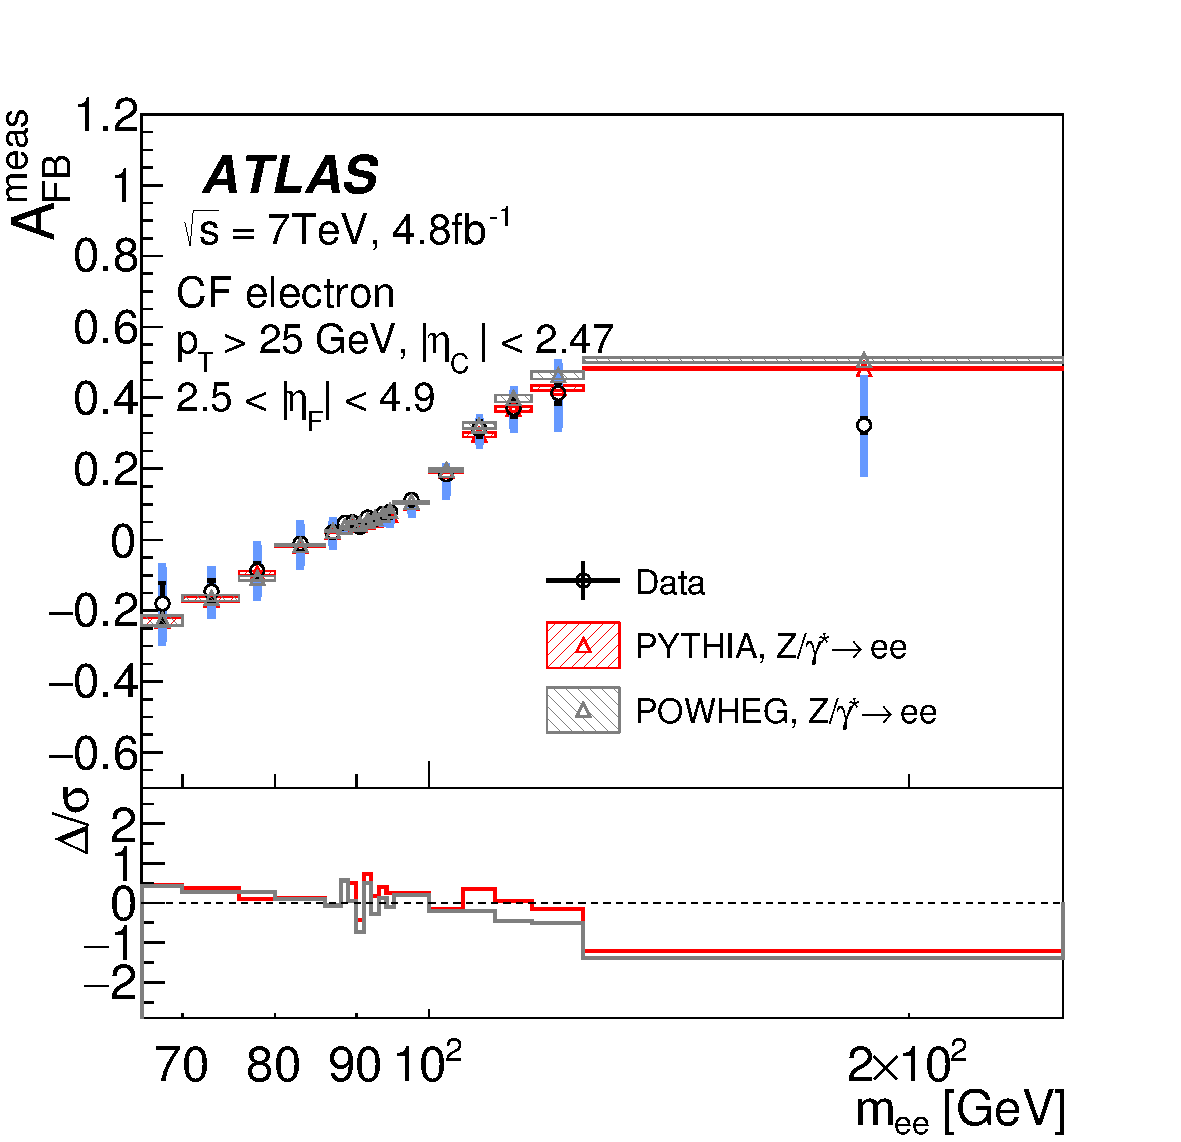
\includegraphics[width=0.45\textwidth]{figures/ss-precision-afb-atlas-cf-afb.pdf}
    \caption{
    From the ATLAS analysis of the full 7 TeV dataset~\cite{Aad:2015uau} on the left: The $\cos\theta^*$ distribution for selected central-forward electron pairs, compared with MC predictions.
    Right: $A^{\rm meas}_{FB}(m)$ for central-forward electron pairs, compared with MC predictions using the best fit $\sin^2\theta^{eff}_{W}$.}
    \label{fig:ss-precision-afb-atlas-cf}
\end{figure}

\begin{figure}[p]
    \centering
    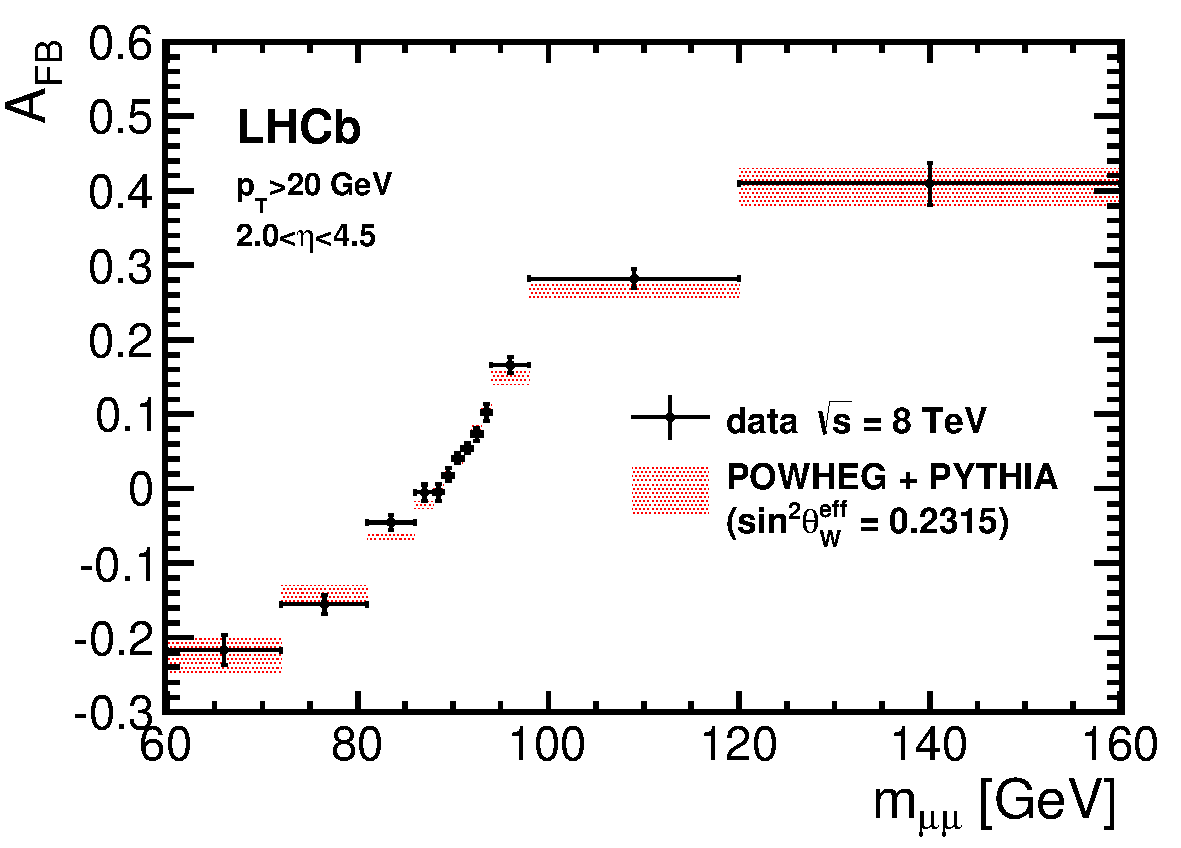
\includegraphics[height=0.3\textheight]{figures/ss-precision-afb-lhcb.pdf}
    \caption{The
unfolded $A_{FB}$ distribution from LHCb 8 TeV data , as a function of di-muon mass, compared with NLO predictions from \texttt{POWHEG-BOX}~\cite{Aaij:2015lka}.
    }
    \label{fig:ss-precision-afb-lhcb}
\end{figure}

\begin{figure}[p]
    \centering
    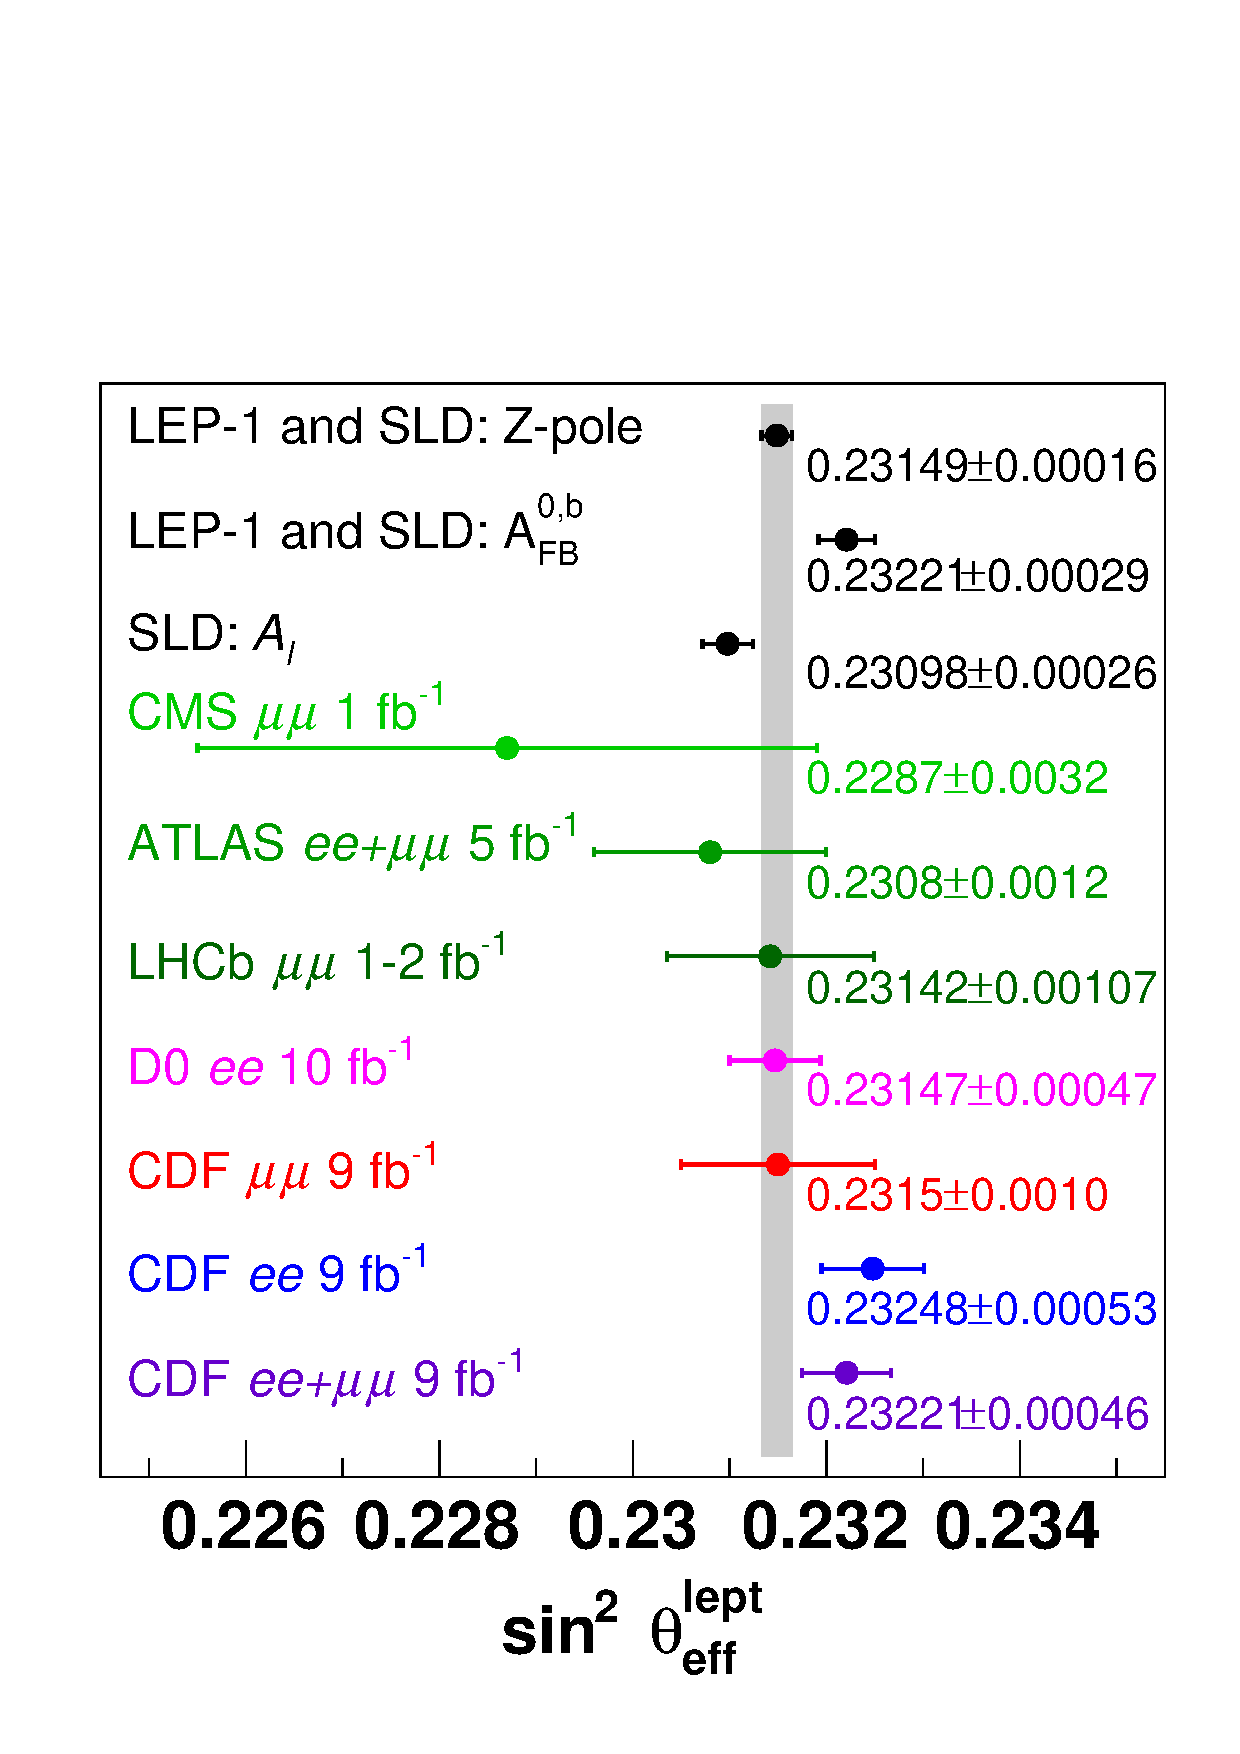
\includegraphics[height=0.3\textheight]{figures/ss-precision-summary-sin2thetaw.pdf}
    \caption{Comparison of experimental measurements of
$\sin^2\theta^{eff}_{W}$~\cite{Aaltonen:2016nuy}.}
    \label{fig:ss-precision-summary-sin2thetaw}
\end{figure}




\subsection{W mass}

\section{Summary}


ATLAS~\cite{Aad:2008zzm}
CDF~\cite{Abulencia:2005ix}
CMS~\cite{CMSdetector}
D0~\cite{Abazov:2005pn}
LHCb~\cite{Alves:2008zz}

CDF Z asymmetry muon~\cite{Aaltonen:2014loa}
CDF Z asymmetry electron~\cite{Aaltonen:2013wcp}
CDF W mass PRD~\cite{Aaltonen:2013vwa}
CDF W mass PRL~\cite{Aaltonen:2012bp}

D0 W asymmetry electron~\cite{Abazov:2013dsa}
D0 W asymmetry muon~\cite{Abazov:2013rja}
D0 W mass PRD~\cite{D0:2013jba}
D0 W mass PRL~\cite{Abazov:2012bv}

CDF+D0 W mass combination~\cite{Aaltonen:2013iut}

Snowmass electroweak~\cite{Baak:2013fwa}

Wmass PDF~\cite{Bozzi:2011ww}

\ack
Acknowledgments go here.

\bibliographystyle{iopart-num}
\bibliography{ewkrun1_master}

\end{document}
